%%%%%%%%%%%%%%%%%%%%%%%%%%%%%%%%%%%%%%%%%%%%%%%%%%%%%%%%%%%%%%%%%%%%%%
% How to use writeLaTeX: 
%
% You edit the source code here on the left, and the preview on the
% right shows you the result within a few seconds.
%
% Bookmark this page and share the URL with your co-authors. They can
% edit at the same time!
%
% You can upload figures, bibliographies, custom classes and
% styles using the files menu.
%
%%%%%%%%%%%%%%%%%%%%%%%%%%%%%%%%%%%%%%%%%%%%%%%%%%%%%%%%%%%%%%%%%%%%%%
\documentclass[12pt]{article}
\PassOptionsToPackage{hyphens}{url}\usepackage{hyperref}
\usepackage{sbc-template}

\usepackage{graphicx,url}

%\usepackage[brazil]{babel}   
\usepackage[utf8]{inputenc}  


     
\sloppy

\title{ADA - Atribuição de Aulas}

\author{Ana Paula Moura Messias de Souza, Gustavo Santos Costa Soares, Henrique Luis Baesa, 
\\Isabella Valerio Mazará, Josineudo das Chagas Arruda, Paulo Kenji Yokota Muneischi}

\address{Instituto Federal de Educação, Ciência e Tecnologia de São Paulo
  (IFSP)\\
  São Paulo – SP – Brasil
\nextinstitute
  Curso Técnico em Informática Integrado ao Ensino Médio
  \\PDS - Pratica para Desenvolvimento de Sistemas 
  \email{ada.ifsp@gmail.com}  \email{{ moura.a,santos.soares,h.baesa,i.mazara,josineudo.c, paulo.muneischi}}
  \email{@aluno.ifsp.edu.br}
}

\begin{document} 

\maketitle

\begin{abstract}
  This document describes the final delivery of the Assignment of Classes (ADA) web application project, developed in the Practical for Systems Development (PSD) course at the Federal Institute of Education, Science and Technology - São Paulo Campus. The ADA aims to automate the aforementioned attribution system, in order to provide ease and agility to the employees involved. Therefore, the target audience are professors and other positions responsible for the general administration and for the representation of each block when configuring the necessary details in the execution of the processes. Keywords: assignement of classes, automation, IFSP-SPO, teachers, regulations, FPA.
\end{abstract}
     
\begin{resumo} 
  Este documento descreve a entrega final do projeto da aplicação \textit{web} \textbf{Atribuição de Aulas (ADA)}, desenvolvido na disciplina Prática para Desenvolvimento de Sistemas (PDS) no Instituto Federal de Educação, Ciência e Tecnologia - Câmpus São Paulo (IFSP-SPO). A ADA visa automatizar o referido sistema de atribuição do instituto, de modo a proporcionar facilidade e agilidade aos funcionários envolvidos. Logo, o público-alvo são os docentes e os demais cargos responsáveis pela administração geral e pela representação de cada bloco ao configurarem os detalhes necessários na execução dos processos. Palavras-chave: atribuição de aulas, automatização, IFSP-SPO, docentes, regulamentos, FPA.
\end{resumo}

\section{Introdução}
\par O sistema de atribuição do IFSP-SPO envolve um processo complexo, porém essencial, para a designação dos docentes em suas futuras aulas, garantindo o cumprimento de sua carga horária e, por conseguinte, a realização efetiva de suas responsabilidades. É conduzido semestralmente, a cada seis meses, com exceção das disciplinas de cursos integrados e PROEJA\footnote{Programa Nacional de Integração da Educação Profissional com a Educação Básica na Modalidade de Educação de Jovens e Adultos}, que ocorrem a cada dois semestres. E, desde 2021, o processo leva cerca de dois meses para ser efetuado e efetivado por completo.
\par Para isso, é seguido o regulamento vigente, a Portaria nº SPO.071, de 15 de março de 2023, que abarca todas as orientações e está embasada na Resolução IFSP nº 112/2014, de 07 de outubro de 2014, alterada posteriormente pela Resolução IFSP nº 109/2015, de 04 de novembro de 2015. Além de serem seguidos o Parecer nº 146/2015/CONSUL/PEIFSÃOPAULO/PGF/AGU e os da CNE/CEB\footnote{Câmara de Educação Básica do Conselho Nacional de Educação.}, em específico a diretriz nº 5/1997, aprovada em 7 de maio de 1997, responsável pela regulamentação da Lei nº 9.394/96.
\par Devido ao seu elevado grau de complexidade, diversos profissionais estão envolvidos, são eles o Diretor-Geral, os diretores de departamento, os coordenadores de curso superior, os representantes de subárea, os docentes, e os diretores de departamento, de ensino e de pesquisa, extensão e pós-graduação. Ademais, os órgãos envolvidos são a Coordenadoria de Turnos (CTU), a Diretoria de Ensino (DEN) e a Diretoria de Pesquisa, Extensão e Pós-graduação (DPE)\footnote{ As atribuições e responsabilidades desses envolvidos são descritas na Portaria, juntamente com todos os procedimentos necessários, localizada no anexo --.}.
\par Atualmente, para a execução do sistema, o processo é executado através de documentos estruturados manualmente e disponibilizados no ambiente virtual eadcampus; a atribuição, em particular, através de múltiplas planilhas detalhadas do Excel. E, na resolução dos conflitos decorrentes de insatisfações individuais, escassez de aulas aos docentes remanescentes, divergências de horários e afins, são realizadas negociações extraoficiais.
\par Ciente da complexidade, a ADA visa automatizar a atribuição, em específico os procedimentos do Art. 3º da Portaria, parágrafos I, II, III, IV, V, VI, VIII, IX e XI. Isso abrange o estabelecimento dos prazos a serem cumpridos; a configuração do ambiente com os dados necessários sobre os horários, as turmas, as disciplinas e os usuários; a determinação do critério de prioridade dos docentes para a atribuição; a realização e entrega do Formulário de Preferência de Atividades (FPA)\footnote{Preenche com seus dados pessoais, disponibilidade de horário, prioridades de aulas, atividades de apoio ao ensino e complementação de atividades (modelo no anexo --).}; a atribuição automática e a manual, em caso de conflitos de preferência; e a possibilidade de permuta após a atribuição, se desejado e viável.
\par Nesse contexto, evidentemente, a aplicação \textit{web} considera o regime de trabalho do docente e assegura o cumprimento das leis trabalhistas e dos regulamentos da Instituição. Essas englobam o número máximo de 25 alunos por turma, uma jornada diária não superior a 8 horas, e o respeito à interjornada de 11 horas. Igualmente, aplica as especificidades do cumprimento de regência de aulas mínimo e máximo de cada regime (20 ou 40 horas).


\subsection{Justificativa}
\par O sistema atual de atribuição demonstra eficácia, entretanto, carece de eficiência, evidenciando várias oportunidades de aprimoramento.
No referido Instituto, há mais de 350 docentes, destes, 56 concentrados no Departamento de Informática e Turismo (DIT) – a área onde a ADA foi criada. Todos participam do sistema de atribuição semestral, submetendo os documentos requeridos e passando por esse procedimento. O resultado é uma considerável quantidade de dados a serem avaliados e de pessoas a serem gerenciadas. 
\par Consequentemente, a organização é comprometida, ocasionando desafios na execução dos procedimentos e insatisfações no desenvolvimento e nos resultados do processo; pela parte dos docentes e dos diretores, coordenadores e representantes. Principalmente nos procedimentos que envolvem o FPA, a atribuição e a possibilidade de permuta, são frequentes os relatos referentes a equívocos no preenchimento, atrasos na submissão, excesso de trabalho manual na atribuição, decisões e alterações em estágios avançados, além de conflitos interpessoais gerados e a decorrente necessidade de comunicações particulares constantes entre o representante do bloco e os docentes\footnote{Realizadas por e-mail, mensagens e/ou ligações.}. Isso foi atestado por meio de uma pesquisa oral com os representantes da DIT, André Evandro Lourenço e Leonardo Andrade Motta de Lima, e com os docentes pertencentes a todos os blocos.
\par Em adição, a quantidade de procedimentos exigidos é considerável, exigindo a troca constante de documentos entre os departamentos e a utilização de múltiplos canais de comunicação\footnote{O comunicador Sistema Unificado de Administração Pública (SUAP), o ambiente virtual eadcampus e o e-mail institucional.}, o que prejudica o controle eficiente do que foi feito (ou não), por quem e em que momento, especialmente caso seja necessária a comprovação das ações.
\par Em suma, esses fatores, em conjunto com a intrincada organização necessária para geri-los, tornam o sistema de atribuição exaustivo e contencioso a todos os envolvidos, demandando um tempo e recursos para armazenamento de dados anteriores que poderiam ser reduzidos significativamente.

\subsection{Objetivo}
\par A ADA é uma aplicação \textit{web} que visa aprimorar não apenas a eficácia, mas, também, a eficiência do sistema de atribuição do DIT. Com essa perspectiva, tem como principal objetivo facilitar a vida dos profissionais envolvidos, a partir da redução do tempo de execução do processo e da aprimoração da gestão dos dados e dos usuários, enquanto promove a transparência. 
\par Ao proporcionar um melhor desempenho, almeja aprimorar a organização, possibilitando o acompanhamento mais eficiente dos procedimentos. E, especificamente nos casos de relatos de erros frequentes, a ADA busca implementar os regulamentos de forma mais confiável, estabelecendo uma padronização e restrição às configurações da atribuição. Inclusive, busca reduzir interferências humanas desnecessárias e repetitivas, assim como, reduzir a necessidade de comunicações extraoficiais, com a resolução de conflitos de preferências diretamente através da aplicação. 
\par Além disso, a aplicação pretende tornar a quantidade de procedimentos mais enxuta, por meio da centralização dos principais em um só local, a ADA. Isso permitirá o controle das ações mais eficiente, por garantir de transparência na monitorização tanto do desempenho dos usuários quanto dos procedimentos, e, igualmente, por facilitar a geração de relatórios com dados, comprovações e auditorias. Como adicional, a integração do banco de dados tornará o acesso e o armazenamento de configurações anteriores mais intuitivas e leves.
\par Assim, uma operação que outrora dependia de organização manual e experenciava desafios no gerenciamento, muitas vezes mais suscetível a erros devido à subjetividade humana, será uma operação tecnológica mais limpa e funcional, onde a interferência humana será restrita a funções indispensáveis.



\section{Análise de Concorrência}
\par A análise do mercado de sistemas de atribuição automatizados resultou na identificação de uma aplicação principal, desenvolvida pela Secretaria da Educação do Estado de São Paulo (SED), e de uma aplicação secundária, pelo Sistema Integrado de Gestão (SIG).
\par A da SED abrange toda a rede educacional estadual de São Paulo (SP), e, de acordo com seus registros (vide anexo --), atende a aproximadamente 6 mil docentes. Em resumo, os docentes selecionam a(s) escola(s) e disciplina(s) na(s) qual(is) desejam lecionar, indicando interesse em aulas vagas, livres ou de substituição – em casos de ausência ou afastamento. Essa aplicação se destacou pela sua complexidade e pelo desenvolvimento semelhante ao proposto pela ADA: a atribuição se baseia em uma fila, porém, o critério é estabelecido por um sistema de pontuação; a escolha das escolas é realizada de acordo com a prioridade definida pelo usuário; os diretores têm acesso a todo o processo.
\par Quanto a do SIG, abrange exclusivamente as Escolas Técnicas Estaduais (Etecs). E, por sua vez, essa aplicação foi considerada como secundária, dado que concentra-se no preenchimento e submissão de inscrição e requerimentos de ampliação de carga horária pelos docentes, entretanto, não realiza a atribuição automatizada em si\footnote{Informações disponibilizadas na página da Unidade de Recursos Humanos (URH), vide anexo --}.
\par A equipe da ADA prevê o tratamento de algumas questões presentes na aplicação da SED, como o gerenciamento da manipulação de múltiplas filas. Igualmente, reconhece outros potenciais pontos de atenção, como o atraso causado por longas filas de seleção; a ausência de verificação de componente curricular, que permite docentes sem o nível de escolaridade necessário lecionarem a disciplina; e os erros no processo de pontuação para prioridade de escolha. \cite{g1_2020} \cite{acioli_2021}
\par Ao mesmo tempo também se reconhecem melhorias a serem implementadas, como abranger melhor todos os casos de exceção – como ausência ou afastamento de um docente –, e discutir a possibilidade de alteração da atribuição final pelo Representante ou Administrador. Em relação ao SIG, detalhes adicionais não puderam ser verificados devido à inacessibilidade ao seu tutorial. Porém, a página que permite aos docentes indicar sua disponibilidade de horário é clara (anexo --) e pode servir como um exemplo.
\par Com base no exposto, a ADA se destaca ao subsidiar uma série de ações que permitem a integração de dados e procedimentos de maneira inovadora, especialmente no âmbito de regulamentos do Instituto e na simplificação das fases no sistema de atribuição. E, dado seu público menor, oferece maior organização, análise de feedbacks e tratamento de erros, com a vantagem de proporcionar um contato direto com os usuários para esclarecimento de dúvidas, o bot Adaline e Adam.\footnote{No apêndice A, há uma tabela comparando as aplicações para melhor visualização.}
\par Portanto, a sua implementação considerará as melhores práticas das aplicações com propósitos similares, e, especialmente, as dificuldades que enfrentaram, não se atendo a um ciclo de falhas.
\par Por fim, é importante ressaltar que, por ambas as aplicações (da SED e do SIG) serem direcionadas a clientes específicos, como a ADA, não são consideradas concorrentes diretas, mas, podem servir como fonte de experiência e aprendizado; é mais apropriado considerá-las aplicações com objetivos similares em vez de concorrentes diretas.



\section{Revisão da Literatura}
\subsection{Instituição Federal}
\par Em 1909, foi instaurada a Rede Federal de Educação Profissional, Científica e Tecnológica, com o Decreto nº 7.566, realizado pelo Presidente Nilo Peçanha em resposta à crise econômica e política da época. As instituições de educação profissional da rede se caracterizam por sua estrutura diferenciada, uma vez que foram criadas pela agregação/transformação de antigas instituições profissionais. \cite{celia}
\par O IFSP foi fundado nesse mesmo ano, como Escola de Aprendizes Artífices, e teve seu início efetivo em 1910. O Campus São Paulo foi uma das primeiras escolas, começando provisoriamente como um galpão na Avenida Tiradentes. \cite{CSPhist_2016} 
Transitou por diferentes processos e denominações ao longo dos anos, todavia, manteve o objetivo de oferecer uma formação de qualidade, com a condição de escola pública vinculada à União e, também, o prestígio junto à sociedade paulistana. \cite{CSPsobre_2016}
\par Com o avanço industrial da década de 80, um novo cenário econômico e produtivo se estabeleceu, com o desenvolvimento de novas tecnologias, agregadas à produção e à prestação de serviços. Para atender a essa demanda, as instituições de educação profissional vêm buscando diversificar programas e cursos para elevar os níveis da qualidade da oferta. \cite{mec} Foi nessa época que o Instituto ampliou a sua atuação e seus objetivos oferecendo cursos superiores na Unidade Sede São Paulo. \cite{CSPhist_2016}
\par Posteriormente, foram implementados diversos cursos voltados à formação de tecnólogos na área da Indústria e de Serviços, Licenciaturas e Engenharias. \cite{CSPhist_2016} E, com a Lei nº 11.892, de 29 de dezembro de 2008, o IFSP ganha seu nome oficial, antes Cefet-SP, Centros Federais de Educação Profissional e Tecnológica.
\par Atualmente, o Instituto se localiza na Rua Pedro Vicente, 625, no Bairro do Canindé, além do desenvolvimento das atividades educacionais, abriga a sede da reitoria da instituição. \cite{CSPhist_2016} Sua estrutura organizacional acadêmica é composta por cinco departamentos, de Ciências e Matemática (DCM), de Construção Civil (DCC), de Elétrica (DEL), de Humanidades (DHU), de Informática e Turismo (DIT), e de Mecânica (DME). E, com eles, dedica-se a fornecer Cursos Técnicos (integrado ao médio, concomitante ou subsequente) e de curta duração (extensão), Graduação (Bacharelado, Licenciatura, Tecnologia e Educação à Distância) e Pós-Graduação (especialização e mestrado).Essas informações estão presentes no site do IFSP-SPO, na área Institucional/Cursos.
\par Os docentes são profissionais com experiência na educação básica, na docência superior e também no mercado de trabalho: aptos, portanto, a apresentar exemplos práticos de aplicação da teoria ministrada em diferentes grades curriculares. \cite{IFSP_2022} 
\par Como centro criador de ciência e tecnologia e com a vasta experiência e competência acumuladas em sua extensa trajetória, o IFSP tem capacidade para proporcionar aos seus estudantes uma visão crítica do conjunto do sistema e do processo produtivo e para contribuir com a educação brasileira, praticando a educação como efetivo fator de desenvolvimento humano e social. \cite{CSPhist_2016} 
\subsection{Regulamentos}
\par A criação da Justiça do Trabalho, pelo Decreto nº 1.237, em 1939, e sua posterior regulamentação, em 1940, e instalação, em 1941, trouxe a necessidade do estabelecimento da Consolidação das Leis de Trabalho (CLT). Por sua vez, essa apenas foi oficializada dois anos depois, pelo Decreto-Lei nº 5452, após a luta de juristas para promover a proteção do trabalhador de forma definitiva e unificar a legislação trabalhista já existente no Brasil.
\par É na legislação trabalhista que são estabelecidos os direitos e deveres de empregados e empregadores como, por exemplo, jornada de trabalho, remuneração, férias, aviso prévio, licenças, rescisão de contrato de trabalho, normas de segurança do trabalho e outras regras fundamentais para as relações de trabalho. \cite{PDI}
\par Enquanto, no âmbito da educação, um grupo de educadores conceituados redigiu o Manifesto dos Pioneiros da Educação Nova, em 1932, para conseguir estabelecer um programa de política educacional amplo e integrado. O documento defendia: a educação como uma função essencialmente pública; a escola única e comum, sem privilégios econômicos de uma minoria; formação universitária para todos os professores; ensino laico, gratuito e obrigatório. \cite{mecinst}
\par Apenas no governo de Fernando Henrique Cardoso, em 1995, passou a ter atribuição exclusiva e começou a redigir leis para promover um ensino de qualidade, cumprindo com o proposto no Manifesto. Assim, tem como áreas de competência a política nacional de educação; a educação infantil; a educação em geral, compreendendo ensino fundamental, ensino médio, educação superior, educação de jovens e adultos, educação profissional e tecnológica, educação especial e educação a distância, exceto ensino militar; a avaliação, a informação e a pesquisa educacionais; a pesquisa e a extensão universitárias; o magistério e a assistência financeira a famílias carentes para a escolarização de seus filhos ou dependentes. \cite{mecinst}
\par No IFSP-SPO, os regulamentos trabalhistas e educacionais são aplicados em inúmeras situações, regem cada aspecto do Instituto – além dos seus próprios regulamentos. No entanto, no sistema de atribuição de aulas, há alguns específicos que influenciam diretamente na execução do processo.
\par Quanto a interjornada, o Artigo 66 da CLT determina: Entre 2 (duas) jornadas de trabalho haverá um período mínimo de 11 (onze) horas consecutivas para descanso. \cite{batista2_2021} Seu escopo principal é proporcional o sono ao trabalhador, ainda que se trate de pessoa submetida a jornadas alternadas ou diurnas. \cite{batista_2021}
\par Tratando-se de docentes, exclusivamente, os Pareceres da CNE/CEB são cumpridos, em específico a diretriz nº 5/1997, aprovada em 7 de maio de 1997, responsável pela regulamentação da Lei nº 9.394/96. Nela, confirma-se a atribuição de, no máximo, 8 horas diárias, equivalentes a dez aulas de 45 minutos.
Sobre o sistema de atribuição em si, semestralmente tem a divulgação de uma nova Portaria, com os procedimentos a serem prosseguidos na atribuição, os documentos a serem entregues (e em qual local), os cargos envolvidos e suas respectivas funções, além dos regulamentos e exceções a serem seguidos e considerados. 
\par Por fim, até o momento, rege a Resolução IFSP nº 109/2015, a qual as Portarias se embasam. Nela, estão presentes as alterações no Regulamento de Atribuições de Atividades Docentes, com um maior detalhamento quanto a casos diversos e especificidades do regime de trabalho, das atividades docentes, da distribuição de carga horária, do processo de atribuição e das documentações exigidas para entrega.
\subsection{Automatização}
\par Uma característica definidora da espécie humana é a capacidade de inventar e refinar continuamente ferramentas que ajudam a aliviar os fardos do trabalho \cite{brief1}. Desde muito antes da história registrada, os seres humanos vêm inventando maneiras de simplificar as atividades diárias para aumentar sua produtividade \cite{brief1}.
\par O termo "automatização" foi criado na década de 1940, quando um engenheiro da Ford Motor Company o utilizou para descrever a maior mecanização das linhas de montagem de automóveis \cite{OVH2}, o que proporcionou a diminuição do trabalho braçal. Entretanto, a automatização já existia há muito tempo, seu conceito esteve presente na pré-história, história antiga, início da era comum, renascimento, primeira revolução industrial e na segunda revolução industrial \cite{brief1}, onde o termo foi criado de fato. E atualmente, a automatização continua crescendo em todo o ecossistema de tecnologia de produção em todos os setores e em empresas de todos os tamanhos \cite{IMTS3}.
\par A Automatição de TI, às vezes referida como automatição de infraestrutura, é o uso de software para criar instruções e processos repetíveis para substituir ou reduzir a interação humana com sistemas de TI \cite{RH7}. Ao aplicá-la em fluxos e processos de trabalho, principalmente aqueles que exigem esforço manual, é possível liberar e dedicar mais recursos a tarefas mais estratégicas \cite{FU5}. Dessa forma, a automatização de um processo manual e repetitivo pode trazer uma maior produtividade e disponibilidade \cite{For6} aos funcionários.
\par A automatização executa o trabalho sozinha, não analisa o próprio desempenho e precisa de monitoramento constante. Enquanto a automação também executa o trabalho sozinha e precisa de monitoramento, mas é capaz de analisar o próprio trabalho em tempo real e tomar decisões. \cite{CIT8} No caso do IFSP-SPO, a primeira é preferível, pois proporciona maior flexibilidade, necessária pela constante mudança nos regulamentos e nas agendas e preferências dos docentes. Assim, essa natureza dinâmica exige uma solução que possa se adaptar prontamente a mudanças regulatórias, ajustes de cronograma e modificações nas preferências individuais dos professores.
\par Em vista disso, percebe-se que os seres humanos sempre percorreram um caminho para diminuir esforços; a ADA tem a finalidade de contribuir para esse propósito, simplificando e otimizando o processo de atribuição de aulas. Logo, liberta os envolvidos de tarefas repetitivas e permite que se concentrem em atividades de maior valor agregado. 
\par Consequentemente, o seu desenvolvimento não apenas se alinha com a longa trajetória de automatização da humanidade, mas também representa um passo significativo na melhoria da eficiência e qualidade dos processos educacionais, com uma abordagem flexível que permite maior capacidade de personalização para que a ferramenta seja moldada de acordo com as especificidades do IFSP-SPO, resultando em um sistema de atribuição de aulas que se adapta ao invés de impor limitações.



\section{Identidade}
\par A Atribuição de Aulas\footnote{A logo está no apêndice --}, denominada ADA, teve sua sigla originada tanto da abreviação de seu nome quanto em homenagem à Ada Lovelace | renomada matemática, escritora e considerada a primeira programadora da história\footnote{Ada discorre sobre como a Máquina Analítica poderia ser usada para alavancar o progresso da sociedade e não só realizar meros cálculos, além de em sua última nota, escrever um algoritmo para que a máquina pudesse computar a Sequência de Bernoulli. ()}.
\par Quanto à equipe, denominada Mottarios\footnote{As logos estão no apêndice --}, se demonstrou ao longo do percurso autogerenciável e responsável, demonstrando proatividade em relação às exigências do projeto e dedicação plena à disciplina. A característica central que conduziu ao resultado satisfatório alcançado foi a coesão entre os integrantes, que se mostraram dedicados e colaborativos. 
\par A seguir, serão apresentadas breves descrições individuais dos membros, com a versão completa disponível na página “Sobre” da aplicação.
\begin{itemize}
    \item \textbf{Ana Paula Moura:} apresenta interesse pelas áreas de jornalismo e administração, ainda indecisa sobre a sua carreira. E a sua experiência profissional inclui o desenvolvimento da Plataforma de Eventos no IFSP CodeLab, em 2022. Na ADA, teve como principal responsabilidade as atividades relacionadas ao backend;
    \item \textbf{Gustavo Santos:} busca uma trajetória na área de segurança da informação e disciplinas correlatas, pretendendo seguir uma carreira acadêmica.  E a sua experiência profissional inclui o desenvolvimento da Plataforma de Eventos no IFSP CodeLab, em 2022, e o desempenho na área de mecânica de usinagem, com programação voltada à máquina CNC. Na ADA, atuou como full-stack, com enfoque no desenvolvimento do backend da aplicação e na sua hospedagem;
    \item \textbf{Henrique Baesa:} possui ambições bem definidas para se especializar no campo da inteligência artificial. Como experiência, apresenta certificação pela Universidade de Harvard em Fundamentos da Ciência da Computação, uma medalha na Olimpíada Brasileira de Informática e trabalha como desenvolvedor full-stack. Na ADA, desempenha, principalmente, atividades de backend;
    \item \textbf{Isabella Mazará:} pretende olhar para o abismo da mente humana e espera que ela corresponda o olhar\footnote{Referência à frase de Friedrich Nietzsche, “E você se olhar durante muito tempo para um abismo, o abismo também olhará para dentro de você.”. () Foi um pensador importante à filosofia e serviram de base para Sigmund Freud, criador da psicanálise.}. Logo, seu plano é cursar psicologia e, posteriormente, se especializar em neurociência. E a sua experiência profissional envolve o desenvolvimento da Plataforma de Eventos no IFSP CodeLab, em 2022. Na ADA, atuou como full-stack e seu papel principal foi ser a representante da equipe, concentrando-se em sua organização, na estrutura da ADA, além de tudo que abrange a documentação;
    \item \textbf{Josineudo Arruda:} deseja seguir a carreira da programação, mais precisamente na área de desenvolvimento full-stack e inteligência artificial, além de se interessar por análise de dados. E a sua experiência profissional inclui a participação no IFSP CodeLab e no estágio de Python no Instituto, em 2023. Na ADA, desempenhou um papel full-stack, com enfoque no desenvolvimento de funcionalidades e no front-end, além de ser um dos planejadores das telas;
    \item \textbf{Paulo Muneischi:} possui aspirações na área da programação, principalmente no campo abrangente do desenvolvimento de \textit{softwares} e \textit{websites}, com um grande interesse na área de desenvolvimento de jogos. E a sua experiência profissional inclui o estágio de Python no Instituto, em 2023. Na ADA, suas responsabilidades incluíram a execução de tarefas full-stack, com um foco na lógica e na programação de processos. 
\end{itemize}



\section{Desenvolvimento}
\par Com a finalidade de apresentar uma aplicação em conformidade com os objetivos propostos, é essencial ter em mente as suas funcionalidades, exceções e validações, além da lógica exigida para sua implementação.
Ao longo das entregas do projeto, foi possível estabelecer a proposta inicial da equipe, a prova de conceito (vide apêndice B) a entrega parcial (vide apêndice C) e, por fim, a entrega final.
\par À medida que a ADA é desenvolvida com as tecnologias e ferramentas escolhidas\footnote{vide apêndice D}, são transpostas as ideias e as lógicas de execução em estruturas para garantir uma compreensão mais ampla. O apêndice -- contém um registro abrangente dessas, realizadas pela equipe, incluindo os épicos da aplicação, o modelo de banco de dados, o protótipo, entre outras estruturas relevantes.
\par Quanto ao idioma escolhido, o principal é o português brasileiro – por ser o nativo do Instituto e da maioria de seus membros – e o secundário é o inglês americano – dada sua universalidade e facilidade de acesso em termos de educação e tradução.
\par Por fim, a seguir, as funcionalidades/processos serão detalhadamente apresentados, levando em consideração que funções envolvendo o CRUD (presente em todos os aspectos, inclusive nas funcionalidades) e validações menos complexas serão omitidas.\footnote{Mais detalhes sobre alguns desses processos e sua representação no banco de dados estão disponíveis no apêndice E, por meio de explicações gráficas.}

\subsection{Funcionalidades}
\subsubsection{Divisão de usuários}
\par Como mencionado, o sistema de atribuição engloba diversos profissionais, cada um com funções específicas. Para atingir o objetivo proposto, foi primordial implementar três níveis de usuários. 
\par O primeiro é o Administrador, responsável pela organização das configurações gerais do sistema de atribuição. O segundo, o Representante, que realiza alterações limitadas as configurações de seu(s) bloco(s). E o terceiro, o Professor, cujo acesso é direcionado às suas funções particulares, de seleção de preferências e participação da atribuição. 
\par Cada nível de usuário possui uma visualização distinta das telas e existe a flexibilidade de designar um usuário para mais de um nível, permitindo acesso integrado por um único login (prontuário e senha). São visualizações diferentes das telas para cada, além da possibilidade de um usuário ser designado para mais de um papel e acessá-las por meio de um único acesso (prontuário e senha).
\par Essa abordagem possibilita a centralização dos principais procedimentos, a manutenção das etapas essenciais e a organização mais estruturada do sistema de atribuição.
\subsubsection{Cadastro}
\par O cadastro ocorre a partir da adição de usuários por outros usuários, seguindo uma hierarquia de níveis de acesso. O procedimento é organizado da seguinte maneira: os desenvolvedores adicionarão os Administradores, que terão acesso direto à aplicação; por sua vez, os Administradores adicionarão outros Administradores e os Representantes; e, por fim, os Representantes adicionarão os Professores.
\par Os Representantes e os Professores recém-adicionados receberão um e-mail contendo um link para efetuarem seu cadastro na ADA. Com isso, os seus dados serão integrados aos já armazenados no banco de dados.
\par Essa abordagem distribuída assegura que a tarefa não fique restrita a um único nível de usuário, garantindo o controle adequado dos usuários e o envio do e-mail a todos, sem deixar um usuário de fora.
\subsubsection{Regras}
\par É de suma importância aderir aos regulamentos do IFSP-SPO e do CNE/CEB para manter a legalidade e a integridade da aplicação. Para isso, foram introduzidas algumas regras que abrangem leis e configurações obrigatórias inerentes ao processo. 
\par A regra referente ao Período de Aula (Timeslot) se fundamenta na duração de uma aula. Atualmente, tem a opção de 45 ou 50 minutos. Portanto, foi desenvolvida uma lógica que calcula a diferença entre o início e o fim do horário e a atribui a uma variável, garantindo flexibilidade para futuras mudanças. 
\par A regra referente à Jornada Diária se fundamenta em não exceder o limite de 8 horas diárias de regência de aulas por docente, com a equivalência em quantidade de aulas está na Resolução nº 109/2015, página 9. Além disso, a regra referente à Interjornada se fundamenta na exigência legal de 11 horas de descanso entre duas jornadas de trabalho. Ambas as regras foram validadas na Disponibilidade de Horário do FPA, fornecendo informações corretas para o processo de atribuição e prevenindo uma sobrecarga.
\par Por outro lado, a regra referente à Quantidade de Estudantes se fundamenta no limite de 25 estudantes por turma e, por conseguinte, um docente por turma. A fim de efetivá-la, uma validação na classe Turma (Classs) foi suficiente. 
\par Por fim, as regras referentes ao Regime de Trabalho se fundamentam na duração do regime do funcionário, que podem ser de 20 ou 40 horas, e, assim, estabelecem um limite de regência de aulas. Nesse caso também foram implementadas diretamente no FPA, com validações para a seleção mínima e máxima de células.
\subsubsection{Combos}
\par As combinações de horários, dia e disciplinas, “combos”, são conjuntos de horários sequenciais de um dia, em que está salva a mesma disciplina de uma turma. Essa abordagem resulta na criação de uma classe que engloba dias e horários relacionados a uma ou mais disciplinas, e esses são registrados durante a montagem da grade horária. 
\par Como mencionado anteriormente, essa funcionalidade desempenha um papel significativo na facilitação do processo de atribuição e, igualmente, no preenchimento do FPA.
\subsubsection{FPA}
\par O FPA marca o ponto inicial do processo de atribuição do semestre, uma vez que as configurações necessárias já foram estabelecidas. Seu preenchimento ocorre em duas etapas, a Disponibilidade de Horário e a Preferência de aulas. Na primeira, o docente seleciona o seu regime de trabalho\footnote{20 horas, 40 horas, RDE, Temporário ou Substituto}, determinando os limites mínimos e máximos de carga horária. Em seguida, seleciona os horários nos quais deseja ou pode trabalhar, respeitando os requisitos mínimos de tempo.
\par Após a conclusão dessa etapa, o processo segue à segunda etapa, onde seleciona as disciplinas primárias e secundárias desejadas que estão disponíveis nos horários selecionados anteriormente. A ordem de preferência auxilia na coordenação de atribuição, especialmente em situações de conflitos com as preferências de docentes anteriores na fila.
\par Ao submeter o FPA, as informações são salvas no histórico para referência futura. E, assim, ele desempenha um papel central no processo de atribuição, orientando as escolhas dos docentes e permitindo uma alocação mais eficiente das aulas.
\subsubsection{Fila}
\par As filas determinam a sequência em que os docentes terão suas aulas atribuídas, de acordo com o critério estabelecido pelo Administrador. A sua estruturação é realizada pelos Representantes, em cada bloco, e permite alterar a ordem manualmente caso necessário, apesar do critério. 
\par Cabe ressaltar que um docente pode estar inserido em mais de uma fila, e o processo de atribuição distribuirá as aulas para todas simultaneamente. Então, é possibilitada a equidade, garantindo que os docentes recebam atribuições de acordo com suas preferências, sem dependerem de uma única fila.
\subsubsection{Atribuição}
\par Se inicia com a automática, que tentará atribuir as aulas primárias do docente. Então, em caso de conflito, tentará atribuir as secundárias, a mesma quantidade que deu conflito nas primárias. E, caso também dê conflito ou não seja possível atingir o mínimo de horas para a regência de aulas, passa à atribuição manual, que enviará um e-mail solicitando que selecione outras disciplinas disponíveis em qualquer horário.
\par Nas situações em que o docente atua em mais de um bloco, ele pode estar em lugares diferentes da mesma fila. Para isso, o sistema prioriza as disciplinas primárias, desconsiderando as secundárias, mesmo se forem do primeiro Bloco em que começou a atribuição.
\par O Celery vai auxiliar no agendamento de tarefas, em que uma função pede para mover o docente para o final da fila, caso não cumpra o prazo, dentro de X horas. Se for uma situação de sucesso, o Celery não executa a função e a tarefa agendada é cancelada àquele docente.
\subsubsection{Desativação de docente}
\par A desativação tem como finalidade permitir que um docente não consiga escolher uma disciplina para lecionar caso esteja desativado na mesma. É uma funcionalidade controlada pelo Representante e designada para casos de exceção. Assim, ao selecionar os detalhes do docente, é possível listar a(s) disciplina(s) que o docente será desativado, e ela(s) não ficarão disponíveis na atribuição.
\par Essa funcionalidade vem da ideia de que a aprendizagem do aluno é proporcionada pela atuação apropriada do docente, tanto no âmbito profissional quanto no pessoal.

\subsection{Testes Automatizados}
\par Na execução dos testes unitários e integrados foi empregada a ferramenta Pytest. Eles abarcaram os \textit{apps} User, Timetable, Staff, Common e Attribution, onde foi acordado sobre a prioridade na verificação da execução. Para a realização do procedimento, foram criadas pastas de teste para cada \textit{app}, em virtude do crescimento constante da aplicação. Dentro delas, foram criados arquivos (vide apêndice F, Figura 7) com a implementação de novas funções de teste, a fim de verificar a precisão da execução das funções originais e de confirmar se há o retorno dos resultados esperados. Assim, a ferramenta avaliou a exatidão da saída de dados, como exemplificado no apêndice F, Figura 8 e 9.
\par Nesse contexto, houve a necessidade de criar  classes e funções fictícias (vide apêndice F, Figura 10 e 11) para a preparação dos dados. Vale ressaltar que, embora sejam criadas no banco de dados, as classes são deletadas após a conclusão dos testes, não impactando negativamente no desempenho da aplicação.
\par Conforme atestado pelo Pytest-cov (Code Coverage / Cobertura de Código), a equipe conseguiu cobrir 60\% da ADA (vide apêndice F, Figura 12-14). E, ao longo do processo, foram identificadas falhas (failed), referentes a resultados divergentes em relação ao esperado, e erros (error), referentes a erros nos códigos dos testes. Isso é evidenciado no relatório gerado pela ferramenta, presente no apêndice F, Figura 15-18.
\par Considerando o exposto, foi possível detectar erros nos códigos das funções da aplicação, falhas que comprometeram o seu correto funcionamento, e algumas funções que se provaram inutilizadas e poderiam ser descartadas, como as que remontam à época da Prova de Conceito (PoC).

\section{Considerações Finais}
\par O sistema de atribuição atual do IFSP-SPO claramente evidencia uma necessidade premente de simplificar os procedimentos envolvidos. A proposta da aplicação \textit{web} ADA visa fornecer uma solução por meio de processos abrangentes e robustos, capazes de enfrentar as complexas demandas do sistema. Isso a partir do reconhecimento da importância da educação eficaz e da necessidade de cumprir os regulamentos legais para atender aos direitos dos usuários.
\par Ao longo deste artigo, exploramos esses processos e outros aspectos ligados à ADA, desde sua concepção até sua implementação e testes. Cada etapa trouxe consigo lições aprendidas e melhorias, com a aplicação de mudanças contínuas e correções de erros identificados pela equipe e pelos orientadores.
\par Nesse aspecto, demonstra a maneira como a tecnologia pode beneficiar os usuários sem remover por completo a interferência humana. Os resultados conquistados demonstram a habilidade da equipe de desenvolvimento, que conseguiu criar um sistema autogerenciável e funcional, produzindo bons resultados, mesmo diante dos múltiplos obstáculos.
\par Através dos resultados obtidos, a ADA serve como ponto de partida para desenvolver uma aplicação que englobe todos os procedimentos do sistema de atribuição atual, descritos no Art. 3 da Portaria n° SPO.071. Consequentemente, no futuro, a aplicação poderá possibilitar a permuta de aulas entre os docentes, seja monitorada ou não pelo Representante. Adicionalmente, poderá incorporar mais leis e exceções, como em situações de substituição e afastamento de docentes, e incorporar o FPA completo, manipulando o processo de designação de atividades de apoio ao ensino e componentes complementares.
\par A ADA é o primeiro passo para a aplicação da automatização total do sistema de atribuição no IFSP-SPO, na área de DIT, e, ainda, em outros departamentos.


\section{Referências}

\begingroup
\renewcommand{\section}[2]{}%
\begin{thebibliography}{11}

\bibitem{acioli_2021}
ACIOLI, M. Problemas no sistema de atribuição de aulas prejudicam professores da rede estadual em Mogi. Disponível em: \url{<https://odiariodemogi.net.br/cidades/problemas-no-sistema-de-atribuic-o-de-aulas-prejudicam-professores-da-rede-estadual-em-mogi-1.30131>}. Acesso em: 27 ago. 2023.

\bibitem{batista_2021}
BATISTA, H. Seção III. Dos períodos de descanso. Disponível em: \url{<https://www.jusbrasil.com.br/doutrina/secao/art-66-secao-iii-dos-periodos-de-descanso-clt-comentada/1198086392#LGL_1943_5-1_A.66>}. Acesso em: 27 ago. 2023.

\bibitem{batista2_2021}
BATISTA, H. Artigo 66 do Decreto Lei nº 5.452 de 01 de Maio de 1943. Disponível em: \url{<https://www.jusbrasil.com.br/topicos/10759018/artigo-66-do-decreto-lei-n-5452-de-01-de-maio-de-1943>}. Acesso em: 27 ago. 2023.

\bibitem{CSPsobre_2016}
CAMPUS SÃO PAULO PIRITUBA. Sobre o IFSP. Disponível em: \url{<https://ptb.ifsp.edu.br/index.php/sobre-o-ifsp>}. Acesso em: 27 ago. 2023.

\bibitem{CSPhist_2016}
CAMPUS SÃO PAULO. Histórico. Disponível em: \url{<https://spo.ifsp.edu.br/historico>}. Acesso em: 27 ago. 2023.

\bibitem{g1_2020}
FIGUEIREDO, P.; PAIVA, P. Professores da rede estadual de SP relatam problemas e tumulto no processo de atribuição de aulas. Disponível em: \url{<https://g1.globo.com/sp/sao-paulo/educacao/noticia/2020/01/24/professores-da-rede-estadual-de-sp-relatam-problemas-e-tumulto-no-processo-de-atribuicao-de-aulas.ghtml>}. Acesso em: 27 ago. 2023.

\bibitem{IFSP_2022}
INSTITUTO FEDERAL DE SÃO PAULO. IFSP encerra 2022 com nota máxima em 21 graduações. Disponível em: \url{<https://www.ifsp.edu.br/noticias/3248-cursos-de-graduacao-do-ifsp-sao-avaliados-com-nota-maxima-pelo-mec#:~:text=O%20IFSP%20encerra%202022%20com>}. Acesso em: 27 ago. 2023.

\bibitem{mec}
MINISTÉRIO DA EDUCAÇÃO. Histórico. Disponível em: \url{<http://portal.mec.gov.br/rede-federal-inicial/historico>}. Acesso em: 27 ago. 2023.

\bibitem{mecinst}
MINISTÉRIO DA EDUCAÇÃO. Institucional. Disponível em: \url{<http://portal.mec.gov.br/component/content/article?id=32681:apresentacao>}. Acesso em: 27 ago. 2023.

\bibitem{celia}
OTRANTO, C. Criação e Implantação dos Institutos Federais de Educação, Ciência e Tecnologia – IFETs. RETTA, Rio de Janeiro, N. 1, p. 89-110, jan-jun, 2010. Disponível em: \url{<https://mapadatese.files.wordpress.com/2013/02/criac3a7c3a3o-e-implantac3a7c3a3o-dos-institutos-federais-cc3a9lia-otranto.pdf>}. Acesso em: 27 ago. 2023.

\bibitem{PDI}
PORTAL DA INDÚSTRIA. Legislação trabalhista: entenda tudo sobre leis trabalhistas (CLT). Disponível em: \url{<https://www.portaldaindustria.com.br/industria-de-a-z/o-que-e-legislacao-trabalhista/>}. Acesso em: 27 ago. 2023.

\bibitem{brief1}
Kaufman, M. (2020). A Brief History of Automation. Disponível em: \url{https://www.exelatech.com/blog/brief-history-automation?language_content_entity=en}. Acesso em: 27 ago. 2023.

\bibitem{OVH2}
OVHcloud. O que é automatização?. Disponível em: \url{https://www.ovhcloud.com/pt/learn/what-is-automation/#:~:text=A%20automatiza%C3%A7%C3%A3o%20significa%20a%20substitui%C3%A7%C3%A3o,reduzem%20custos%20e%20o%20stresse}. Acesso em: 27 ago. 2023.

\bibitem{IMTS3}
OVHcloud (2021). A Brief History of Automation Technology. Disponível em: \url{https://www.imts.com/read/article-details/A-Brief-History-of-Automation-Technology---1/1197/type/Read/1}. Acesso em: 27 ago. 2023.

\bibitem{RH4}
Richardson. D (2021). Top 10 reasons to use automation. Disponível em: \url{https://www.redhat.com/en/blog/top-10-reasons-use-automation}. Acesso em: 27 ago. 2023.

\bibitem{FU5}
FindUp (2023). Como a automação de TI pode ajudar sua empresa?. Disponível em: \url{https://www.ovhcloud.com/pt/learn/what-is-automation/#:~:text=A%20automatiza%C3%A7%C3%A3o%20significa%20a%20substitui%C3%A7%C3%A3o,reduzem%20custos%20e%20o%20stresse}. Acesso em: 27 ago. 2023.

\bibitem{For6}
Cameron. P. 5 Benefits of Automation: The Advantages of Automation. Disponível em: \url{https://www.fortra.com/resources/guides/automation-advantages-5-benefits-automation}. Acesso em: 27 ago. 2023.

\bibitem{RH7}
Red Hat (2023). O que é a automação de TI?. Disponível em: \url{https://www.redhat.com/pt-br/topics/automation/whats-it-automation}. Acesso em: 27 ago. 2023.

\bibitem{CIT8}
CentralIT (2021). VEJA COMO NÃO CONFUNDIR AUTOMAÇÃO E AUTOMATIZAÇÃO. Disponível em: \url{https://centralit.com.br/veja-como-nao-confundir-automacao-e-automatizacao/}. Acesso em: 27 ago. 2023.



\end{thebibliography}
\endgroup


\bibliographystyle{sbc}


\section{Apêndices}\label{sec:figs}

\subsection{Apêndice A - Comparação de Aplicações} 

\begin{figure}[h]
    \centering
    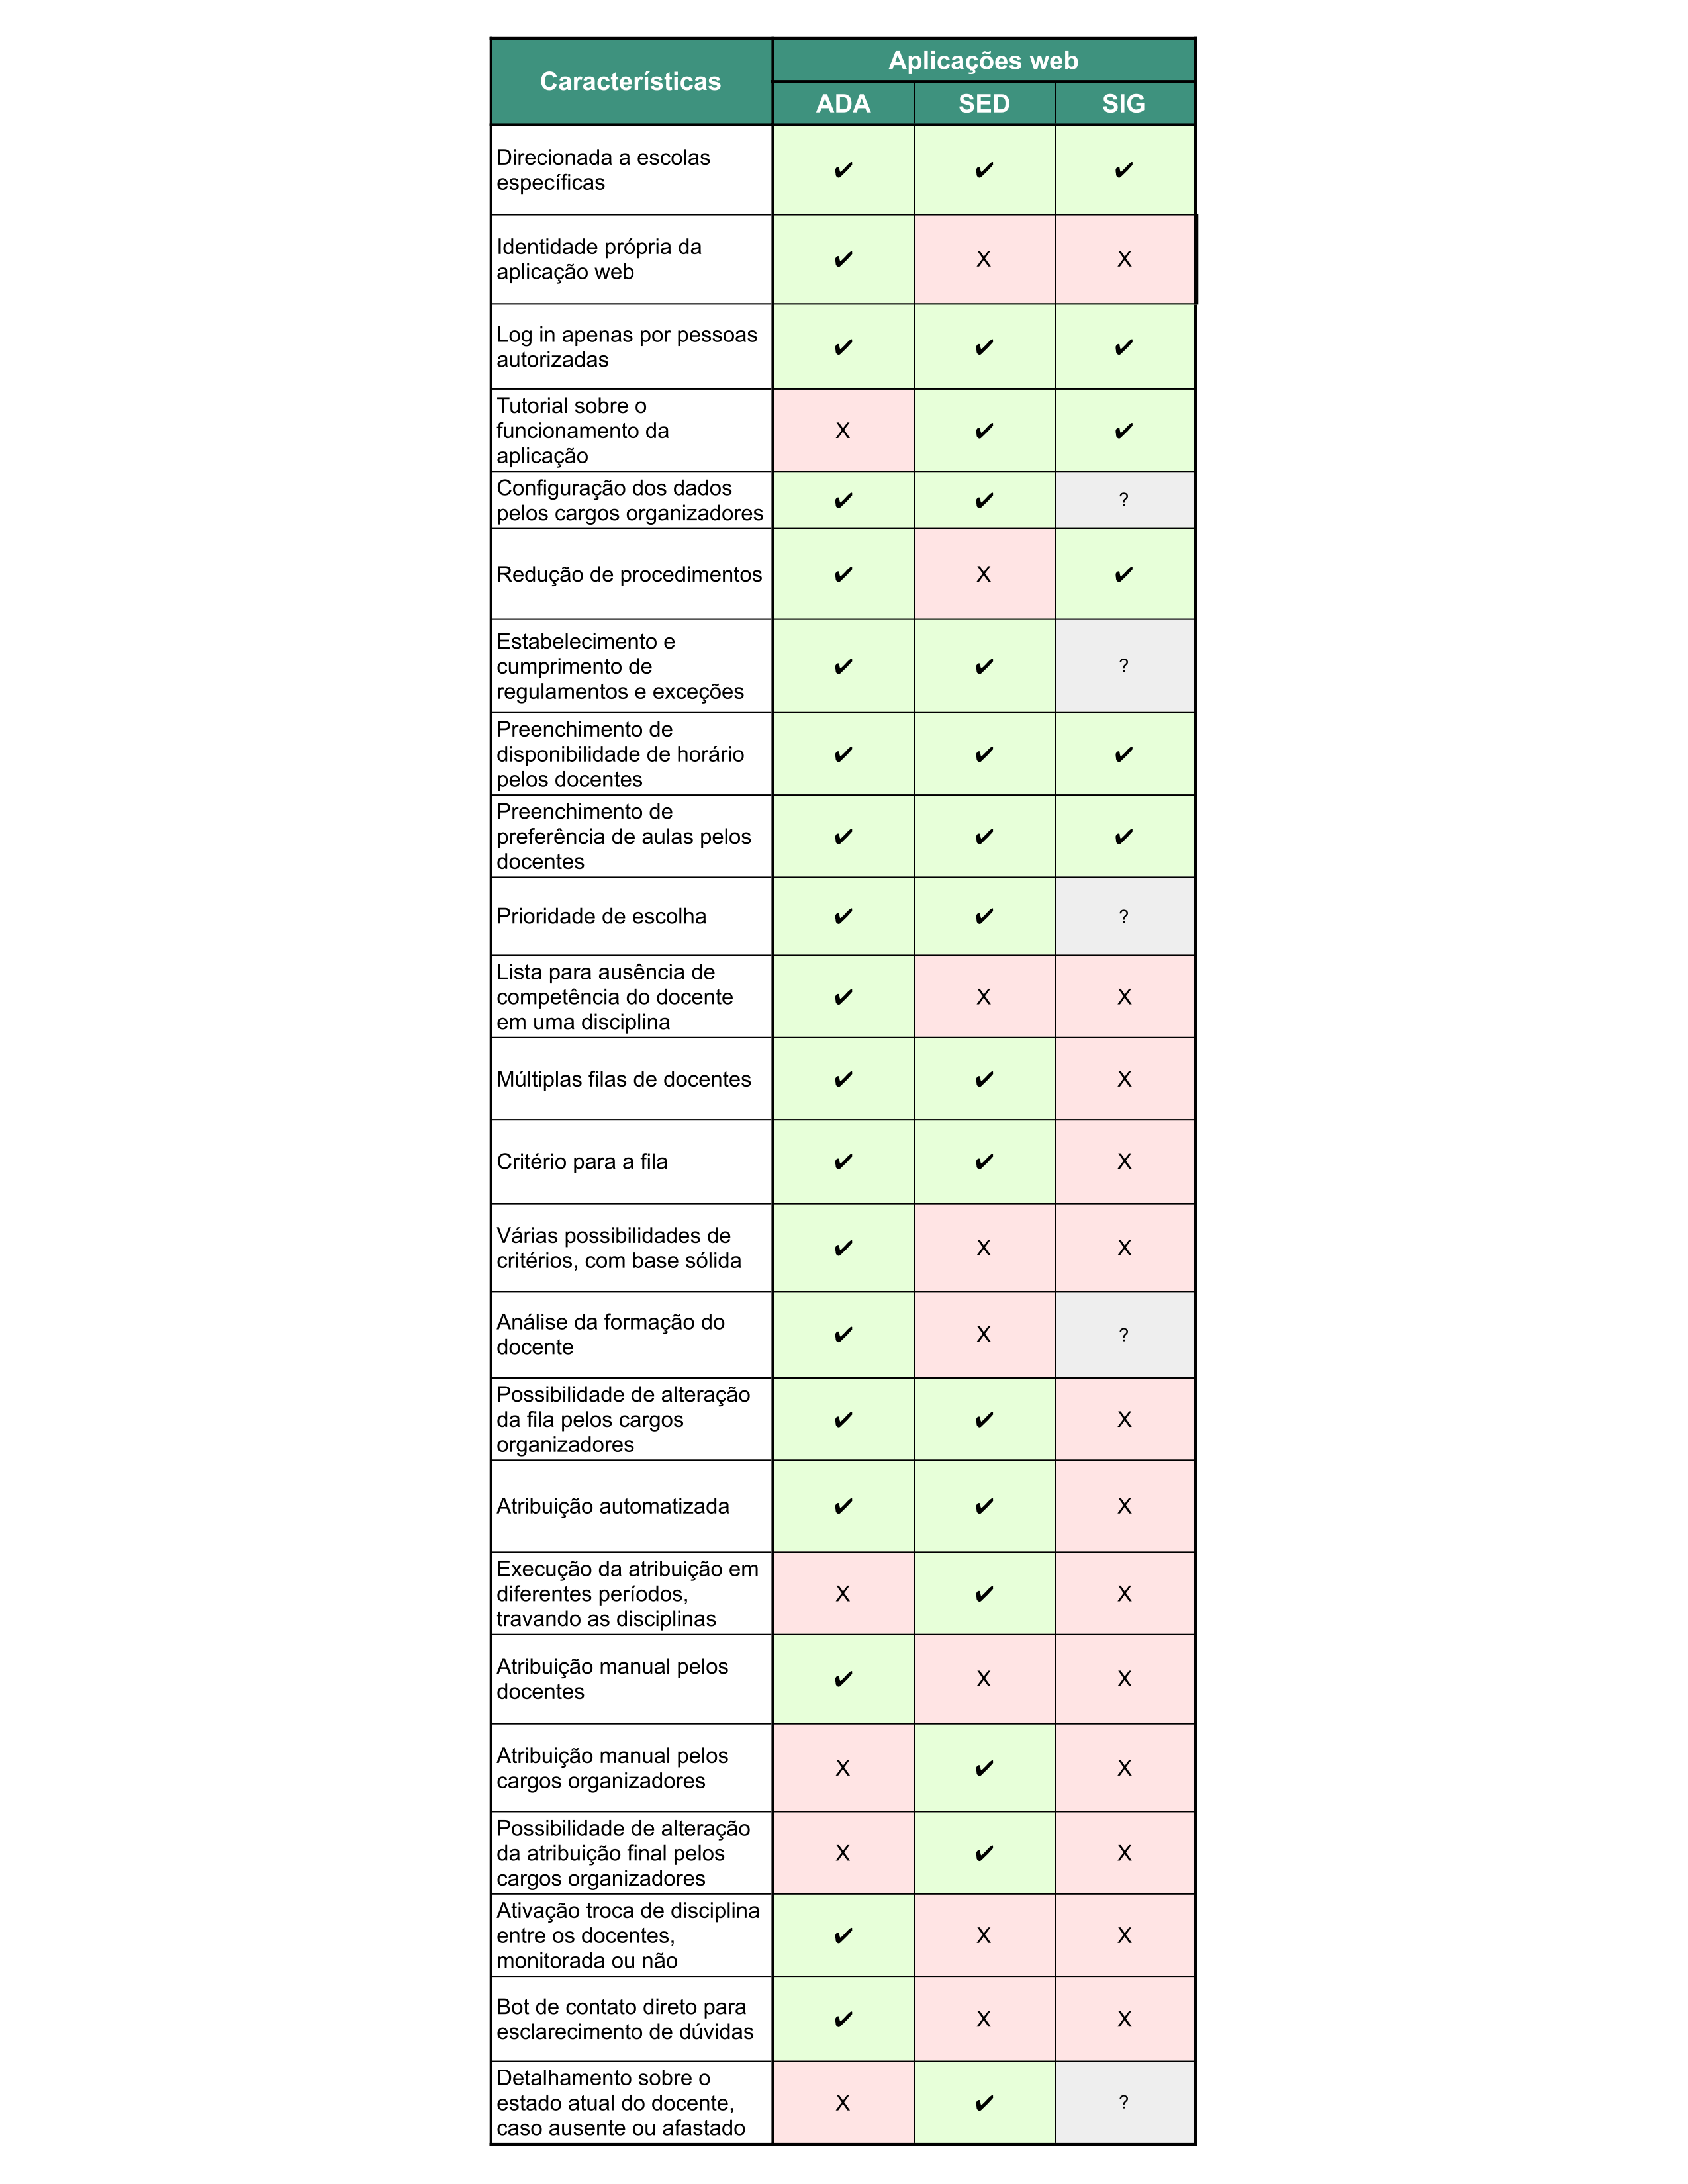
\includegraphics[width=.8\textwidth]{comparacaoaplicacoes.png}
    \caption{Comparação das características apresentadas pelas aplicações na análise de mercado}
    \label{fig:comparacao}
\end{figure}

\subsection{Apêndice B - Detalhes sobre a Prova de Conceito} 
\par A PoC tem como objetivo verificar a viabilidade do desenvolvimento das funcionalidades propostas inicialmente, através das tecnologias, das ferramentas e do tempo disponíveis. Embora não seja necessária uma elaboração detalhada, sua finalidade é demonstrar a capacidade de aplicar a lógica necessária para a construção da aplicação.
\par Nessa etapa, a ADA cumpriu suas metas propostas, entregando tanto o cadastro para usuários autorizadas, quanto o principal, a atribuição de aulas. As obrigações solicitadas foram igualmente atendidas: a internacionalização, a hospedagem e a implementação de criptografia. 
\par No entanto, alguns pontos que requerem atenção mais detalhada foram ressaltados pelos orientadores. Tratam-se da necessidade de compreender como os dados são armazenados no banco de dados e a como as classes se relacionam. A criação de um modelo de banco de dados apropriado foi exigida. Além disso, foram identificadas correções necessárias no diagrama de arquitetura e no tratamento de explicações subjetivas relacionadas à seleção das tecnologias e ferramentas utilizadas, entre outros comentários mais específicos.
\par Em suma, a PoC teve seu objetivo alcançado. A equipe de desenvolvimento da ADA reconheceu a necessidade de fazer alterações nos frameworks utilizados, substituindo o Spring Boot e o Angular pelo Django e Bootstrap, respectivamente, e optou por migrar o sistema de gerenciamento de banco de dados do MySQL para o SQLite3. Quanto aos comentários e observações feitas, foram consideradas e devidamente corrigidas para a entrega subsequente.

\subsection{Apêndice C - Detalhes sobre a Entrega Parcial}
\par A Entrega Parcial desempenhou um papel crucial no desenvolvimento das funcionalidades da ADA. Como comprovado na PoC, a possibilidade de desenvolvê-las foi confirmada e, como resultado, foram efetivamente implementadas.
\par Com a definição oficial da divisão da aplicação em três tipos de usuário, foram entregues diversas funcionalidades: a regra para a determinação dinâmica do período de aula; a grade de aulas com disciplina, horário, período e dias; os combos para sequenciar aulas da mesma disciplina e turma; o preenchimento digitalizado do FPA, em conformidade com os regulamentes vigentes;  a implementação de múltiplas filas de acordo com o critério selecionado e a confirmação do Representante; e a atribuição automática, por meio do software Celery, em conjunto com a atribuição manual, em caso de conflitos de preferências.
\par Diante dos resultados obtidos, a equipe identificou alterações que necessitavam ser implementadas, são elas: os testes exigidos nas regras da disciplina do projeto; a inclusão de validações específicas; e a padronização, melhoria estética e aplicação de responsividade nas páginas.
\par Adicionalmente, a equipe constatou que o período de tempo disponível não permitiu a conclusão de algumas tarefas, como a internacionalização de variáveis, a formulação de regras aos períodos de jornada de trabalho e interjornada, a finalização das páginas destinadas aos docentes, e a reorganização de certas URLs.
\par Durante essa análise dos resultados, também foram identificadas adições benéficas à ADA. Por exemplo, a inclusão de uma aba de notificações, a implementação de uma validação para considerar o período de descanso do docente ao avaliar a possível demora na resposta à atribuição manual, e a busca por melhorias na segurança.
\par As observações dos orientadores, nesta etapa, foram focadas principalmente em detalhes do front-end e sugestões para melhorar a usabilidade. No entanto, pontos críticos foram destacados, como a necessidade de uma pesquisa mais aprofundada sobre o que implementar para melhorar a segurança, a remoção dos alertas de teste que podem expor dados sensíveis aos usuários, a demanda por personalização das páginas de erro para evitar vulnerabilidades na segurança da informação e nortear o usuário sobre o que ocorreu, e a investigação de um erro na atribuição que causa um loop, quando deveria parar após um número determinado de tentativas. Além disso, foi sugerida a implementação do preenchimento automático das células do FPA ao clicar no período, realizada posteriormente.
\par Dado o exposto, essa entrega foi essencial ao amplo desenvolvimento da ADA e, igualmente, à identificação de áreas de aprimoramento necessárias para proporcionar uma aplicação mais sofisticada e, consequentemente, uma experiência mais positiva aos usuários.

\subsection{Apêndice D - Tecnologias e Ferramentas}
\underline{Tecnologias}
\par A ADA é uma Single-page Application (SPA) cuja escolha de tecnologias foi fundamentada em um objetivo central: aprendê-las, dominá-las e implementar a aplicação de forma ágil e eficiente para os desenvolvedores. Isso possibilitou direcionar o tempo à lógica das funcionalidades em detrimento de funções mais básicas, como as operações CRUD (Create, Read, Update, Delete).
\par A linguagem de programação selecionada é o Python, open source e de alto nível, caracterizada por sua forte tipagem dinâmica. Ela se destacou por sua facilidade de compreensão devido à sintaxe concisa e descomplicada, com poucas exigências gramaticais. Para otimizar o desenvolvimento, a escolha recaiu ao \textit{framework web} Django, uma vez que adere ao padrão MTV (Model-Template-View), ao princípio Don't Repeat Yourself (DRY) e ao nível moderável de opinação. Essa combinação de escolhas já demonstrou sucesso no Sistema Unificado de Administração Pública (SUAP) do IFSP, o que facilita a padronização das aplicações utilizadas pelo Instituto.
\par Para promover maior interação entre o cliente e o servidor, o AJAX é empregado em conjunto com a linguagem dinâmica JavaScript, a qual permite renderizar as funções e viabiliza interações locais com o conteúdo da página. Esses recursos são obrigatórios ao desenvolver uma SPA e são particularmente imprescindíveis no desenvolvimento de funcionalidades como o FPA. 
\par Outro framework empregado é o Bootstrap, utilizado para a estilização das páginas. Isso simplifica a estilização e garante a responsividade aos desenvolvedores. Para suporte adicional em casos em que não abrange detalhes específicos, recorre-se ao Cascading Style Sheets (CSS).
\par Quanto ao armazenamento dos dados, optou-se pelo Sistema de Gerenciamento de Banco de Dados (SGBD) SQLite3, por sua capacidade de incorporar o banco de dados diretamente na aplicação (é embutido), eliminando a necessidade de um servidor dedicado, o que está em sintonia com o padrão MTV. 
\par O comportamento da união dessas tecnologias é representada no Diagrama de Arquitetura a seguir:
\begin{figure}[h]
    \centering
    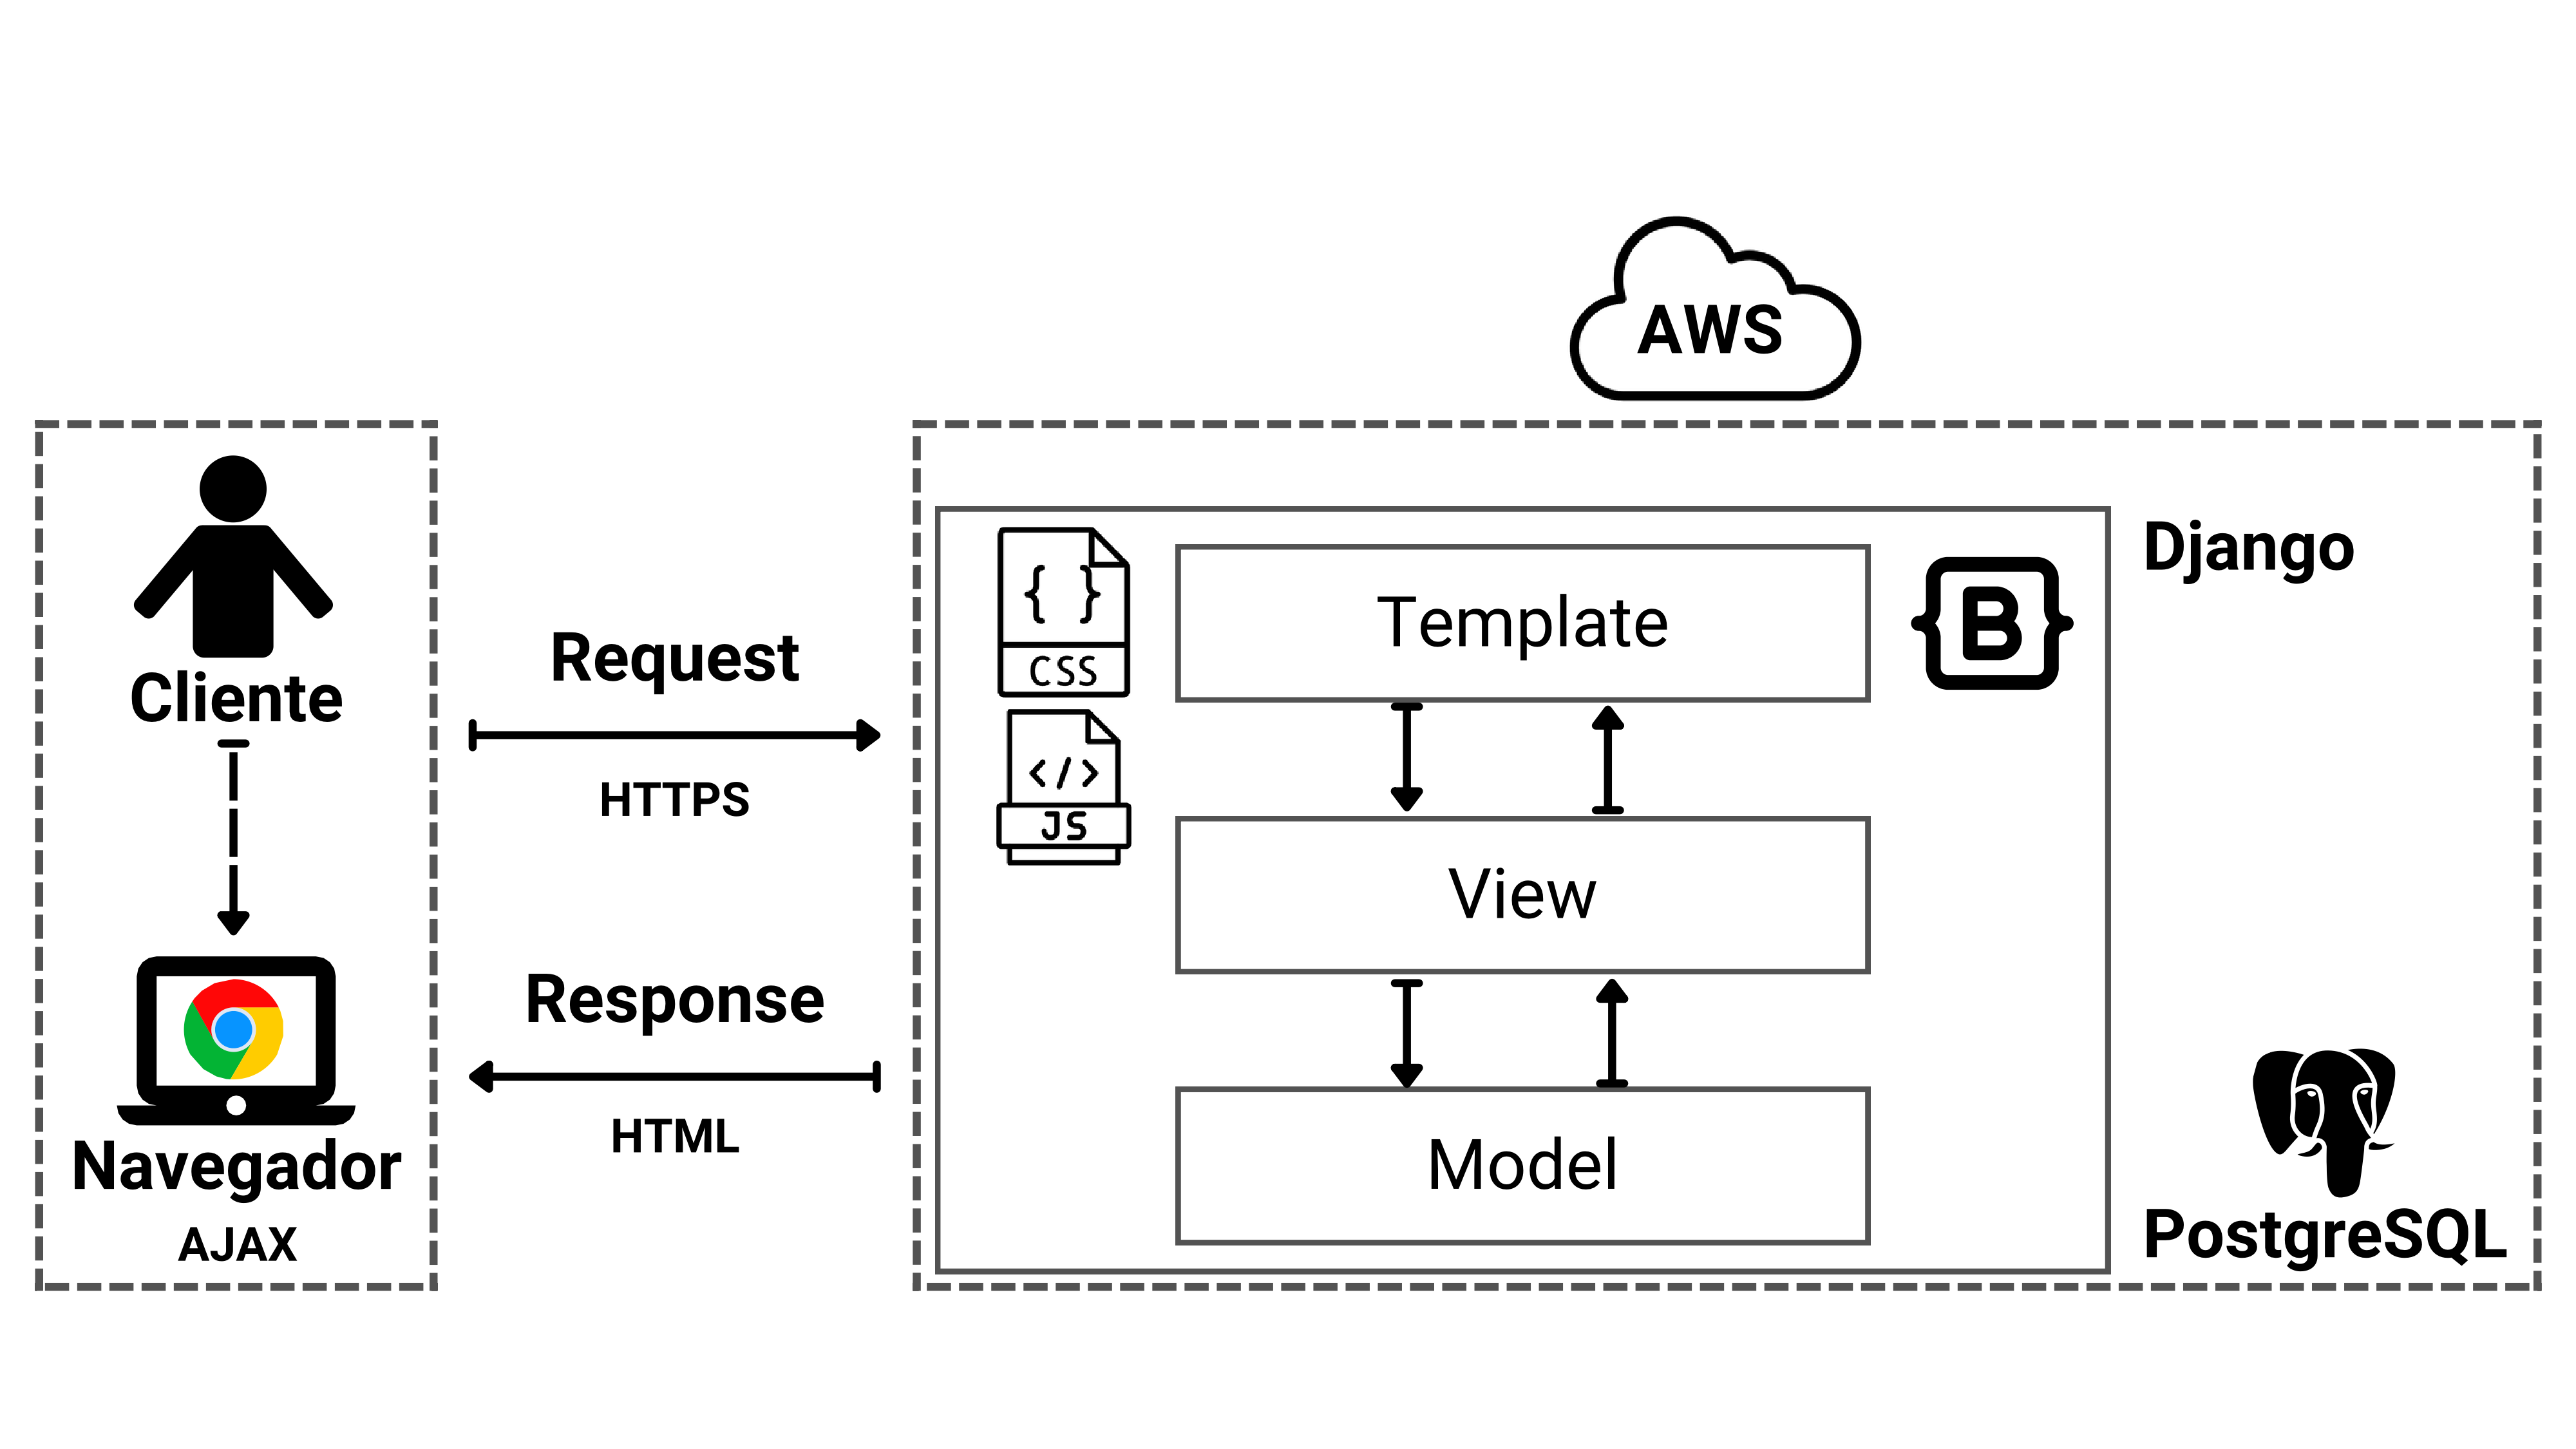
\includegraphics[width=0.9\textwidth]{diagramaarquitetura.png}
    \caption{Diagrama de arquitetura da ADA}
    \label{fig:diagrama}
\end{figure}
\par Por fim, a hospedagem é realizada através da \textit{Amazon Web Services}/Serviços \textit{Web} da Amazon (AWS), para garantir o funcionamento ininterrupto da aplicação, independente de um computador pessoal estar constantemente conectado. Além disso, para aprimorar a identificação, adquiriu-se o domínio https://mottarios.cloud/ por meio da Hostinger, já configurado com o protocolo de segurança HTTPS e com avaliação de nota A pelo Secure Sockets Layer (SSL) Labs.

\par \underline{Ferramentas}
\par No decorrer do desenvolvimento do projeto, foram escolhidas algumas ferramentas com base na familiaridade dos desenvolvedores e em sua conveniência. 
No que diz respeito ao controle de versões, o TortoiseSVN foi adotado devido à sua organização e segurança, uma vez que já havia sido utilizado em projetos dos anos anteriores na disciplina. Adicionalmente, o GitHub foi escolhido devido à familiaridade e à capacidade de gerenciamento aprimorado dos códigos por meio de branches.
\par Em relação à documentação, o Overleaf é empregado para manipular os padrões SBC e ABNT com facilidade para os desenvolvedores, possibilitando o compartilhamento e a edição simultânea.
\par Quanto à programação, a ferramenta escolhida é o Visual Studio Code (VSCode), devido à sua leveza, ao favorecimento da produtividade, por meio do recurso IntelliSense, que a Microsoft recomenda por ajudar “[...] a manter o acompanhamento dos parâmetros que está digitando e a adicionar chamadas a métodos e propriedades pressionando apenas algumas teclas; e comandos para atalhos.”. E, novamente, à familiaridade que os membros da equipe já possuem com essa ferramenta.

\subsection{Apêndice E - Detalhes Funcionalidades}
\begin{figure}[h]
    \centering
    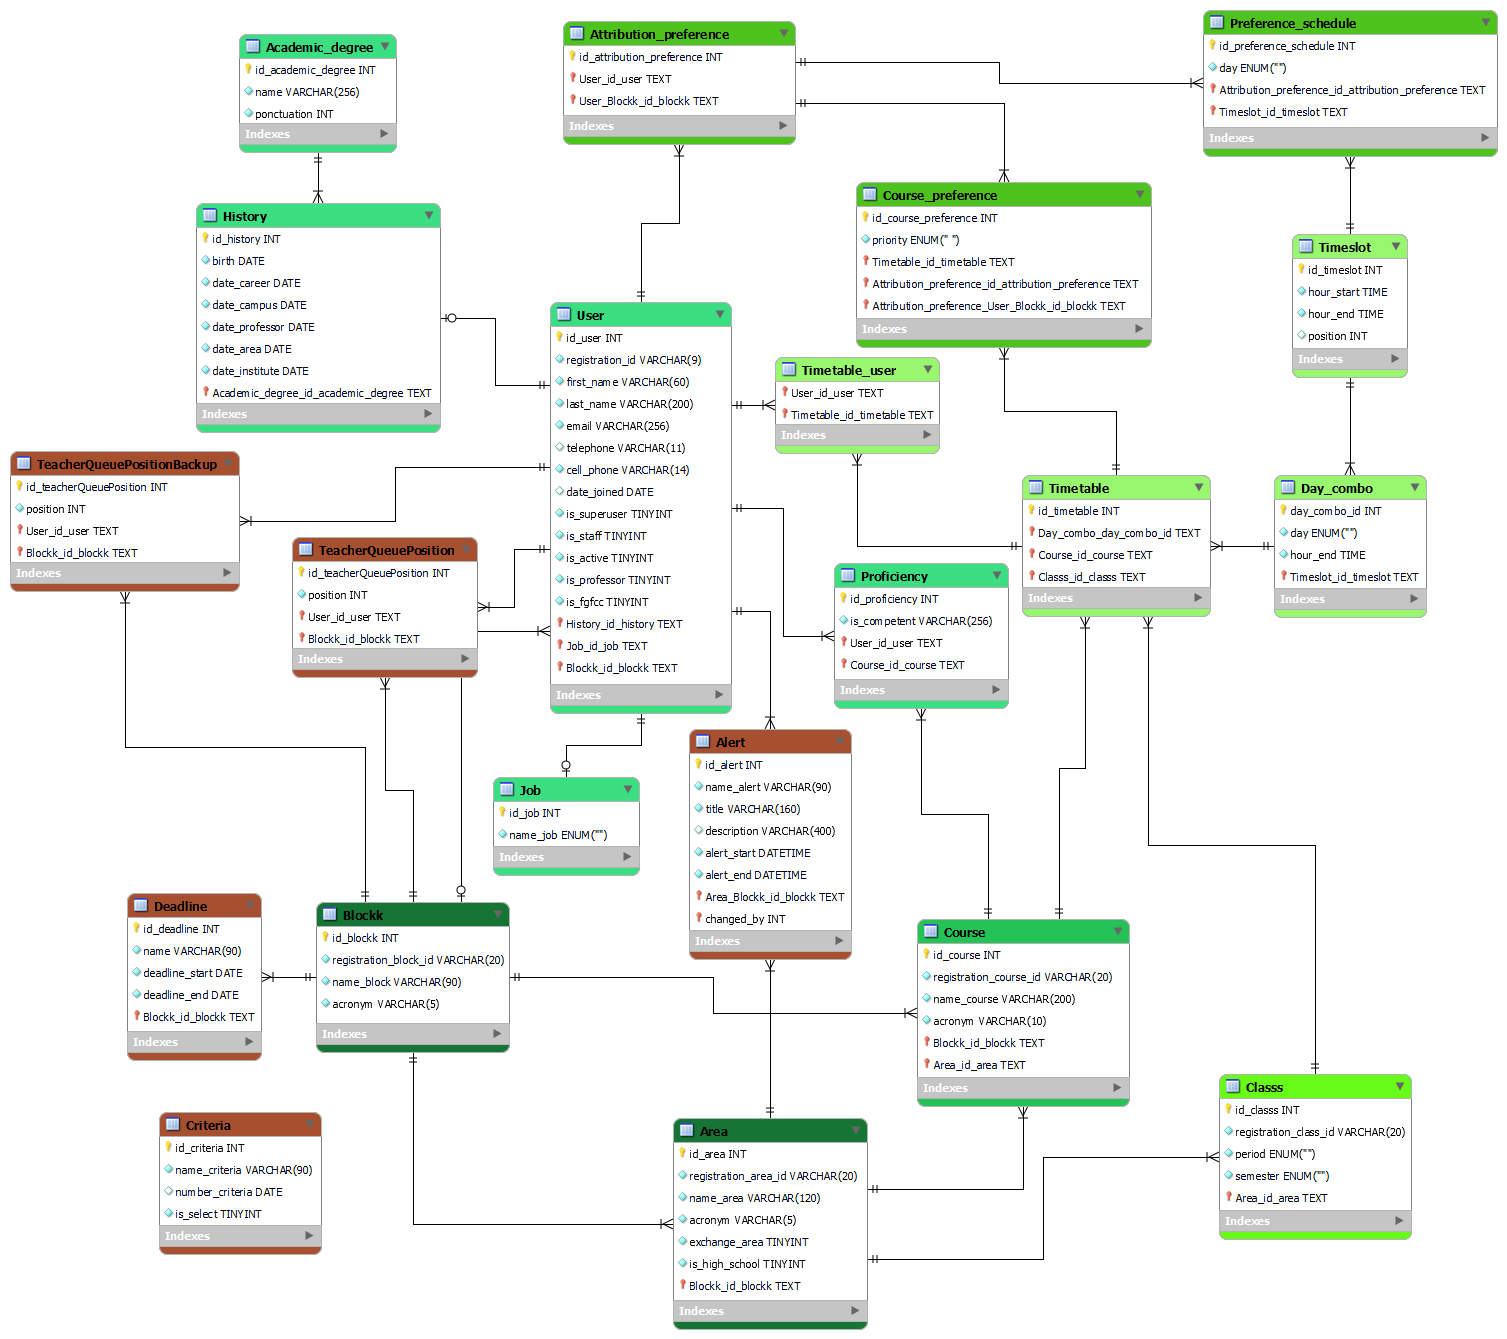
\includegraphics[width=0.9\textwidth]{modelobanco.png}
    \caption{Modelo de banco de dados da ADA}
    \label{fig:bd}
\end{figure}
\begin{figure}[h]
    \centering
    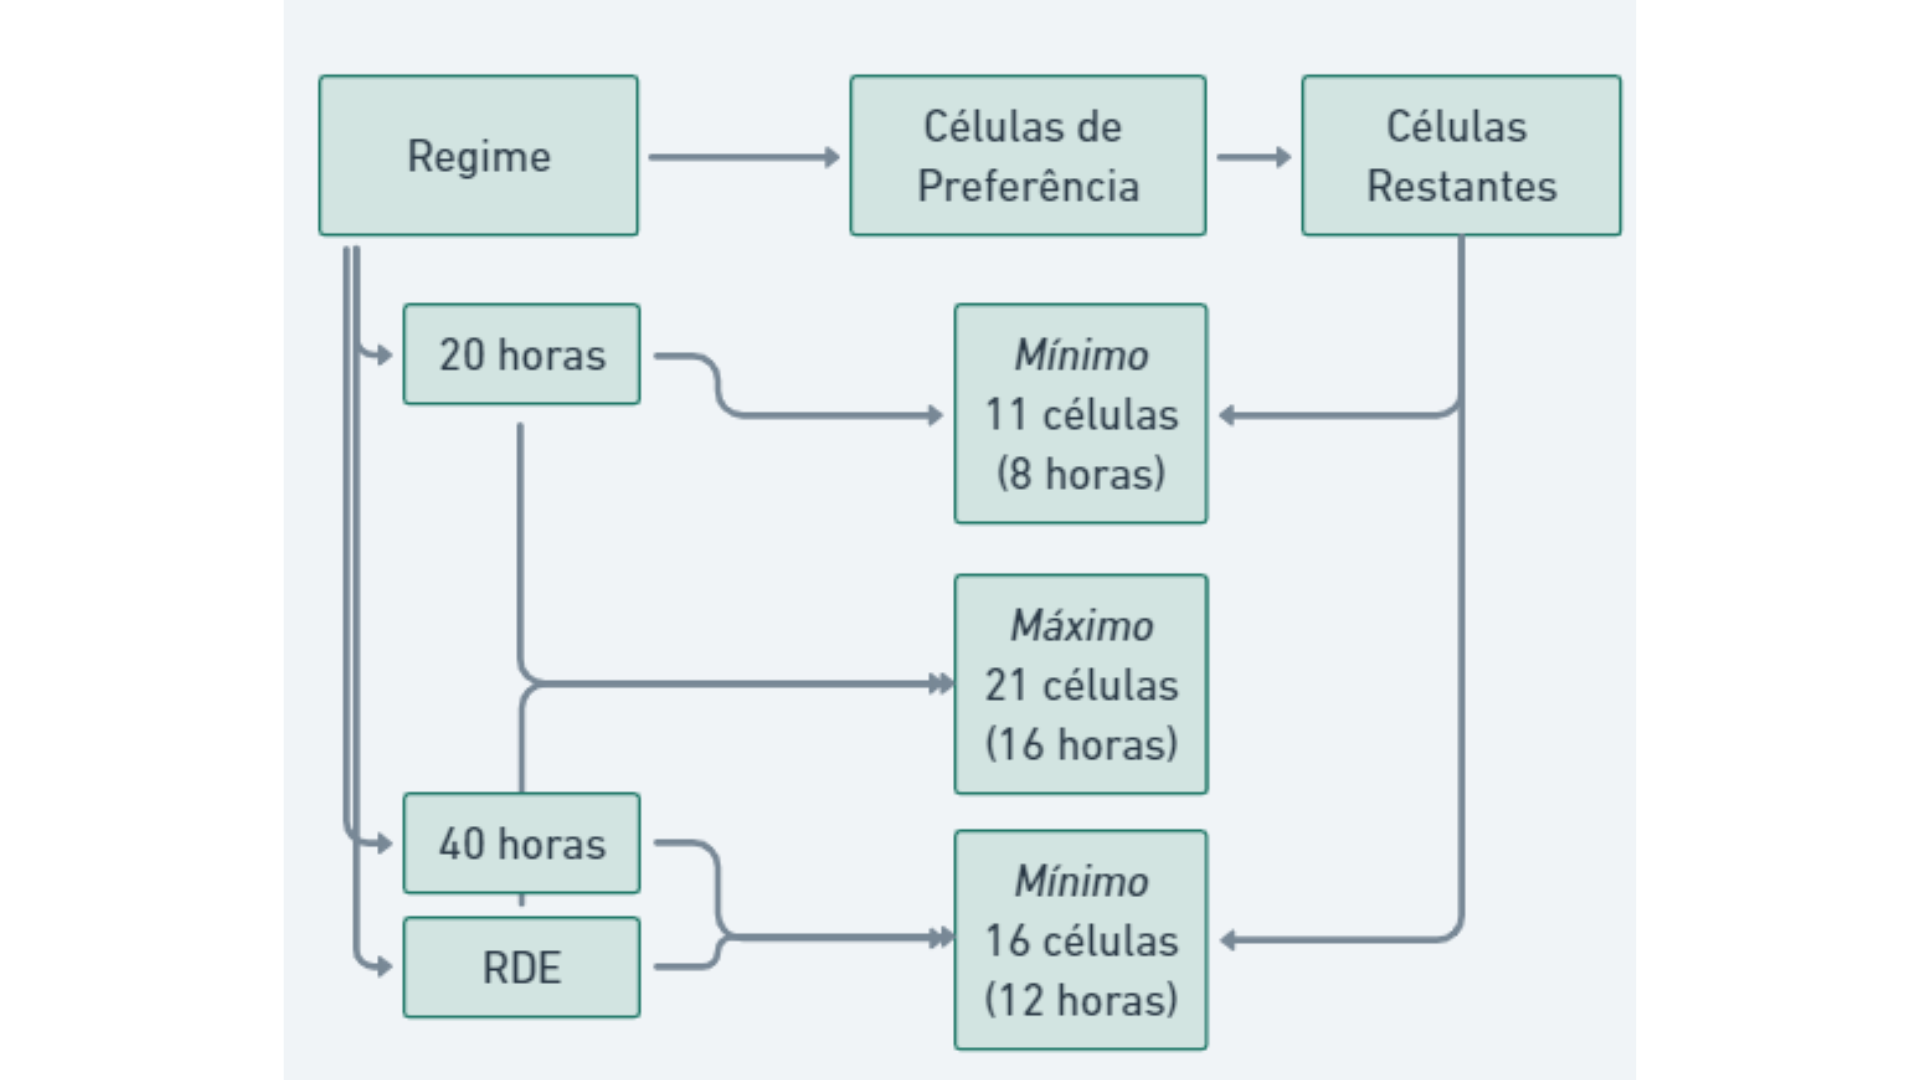
\includegraphics[width=0.8\textwidth]{regras.png}
    \caption{Regras quanto ao regime do docente}
    \label{fig:bd}
\end{figure}
\begin{figure}[h]
    \centering
    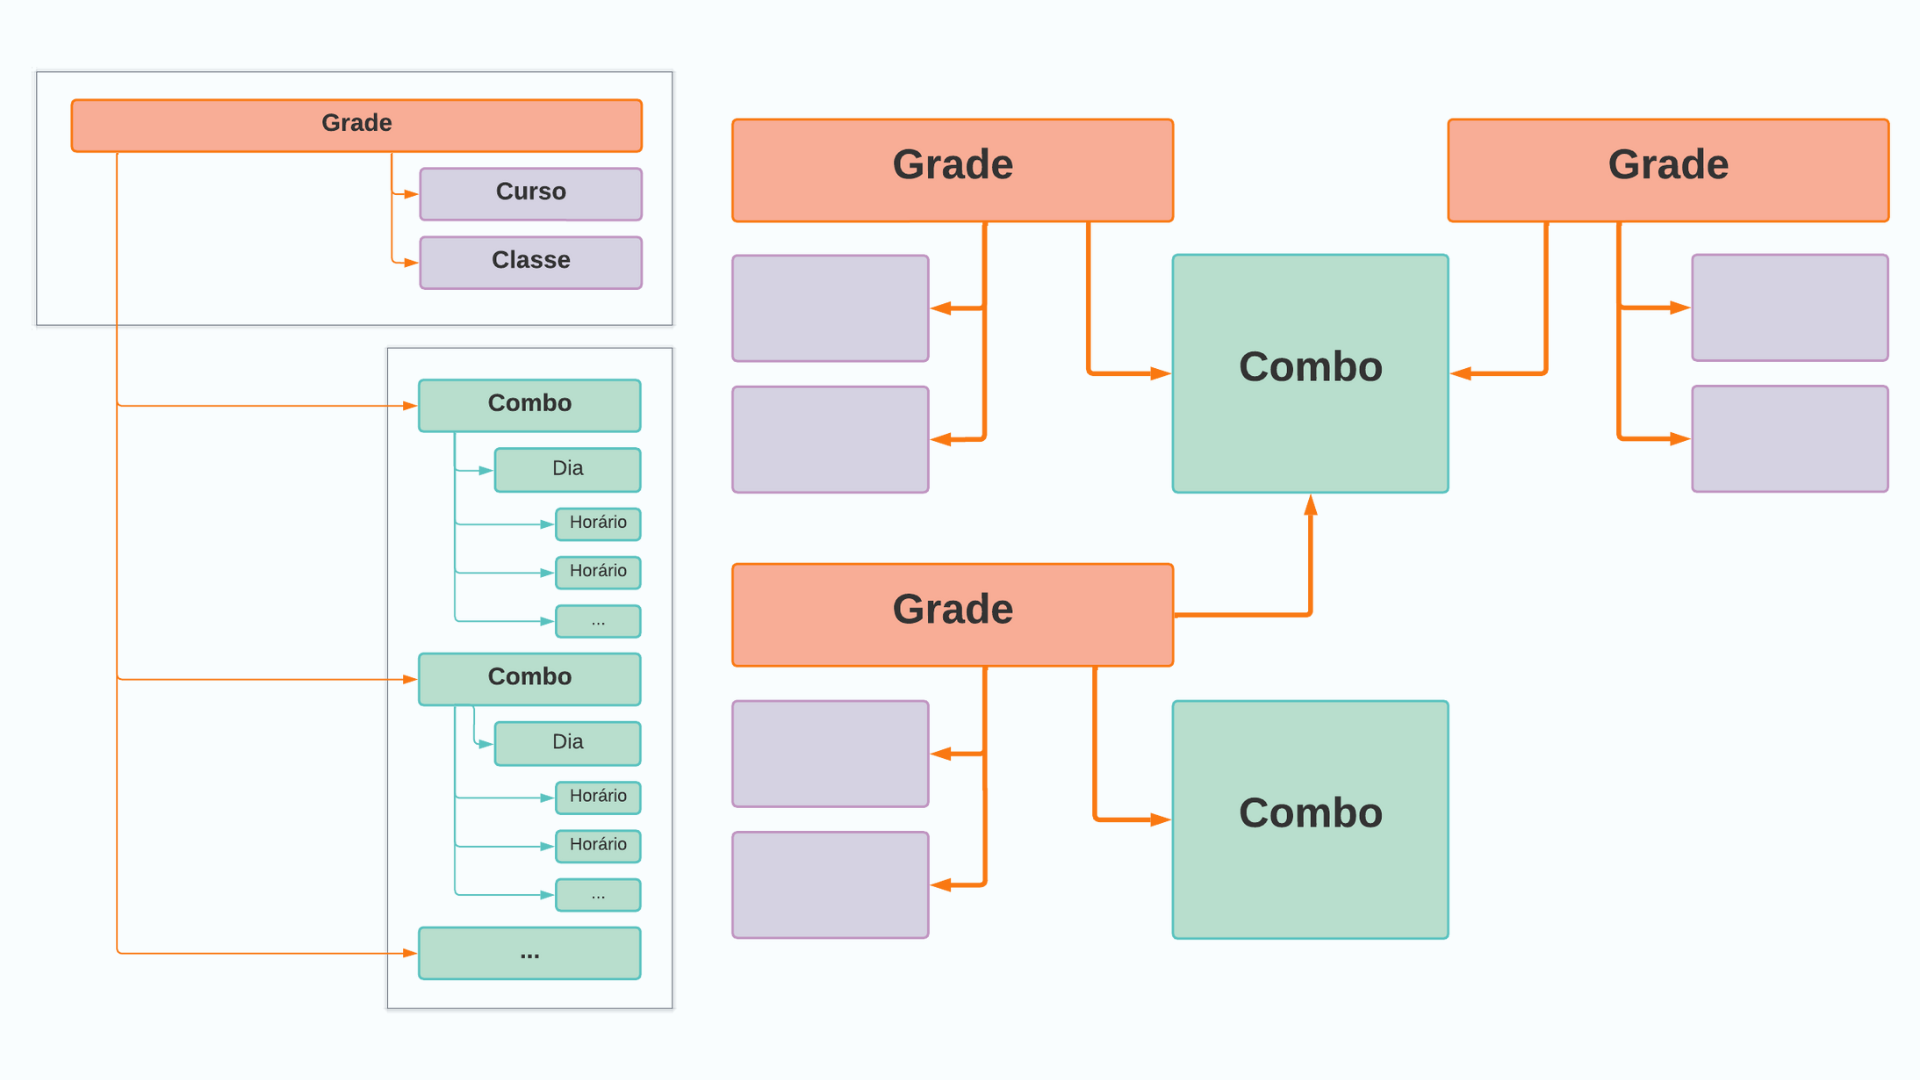
\includegraphics[width=0.6\textwidth]{combos.png}
    \caption{Representação gráfica dos combos}
    \label{fig:bd}
\end{figure}
\begin{figure}[h]
    \centering
    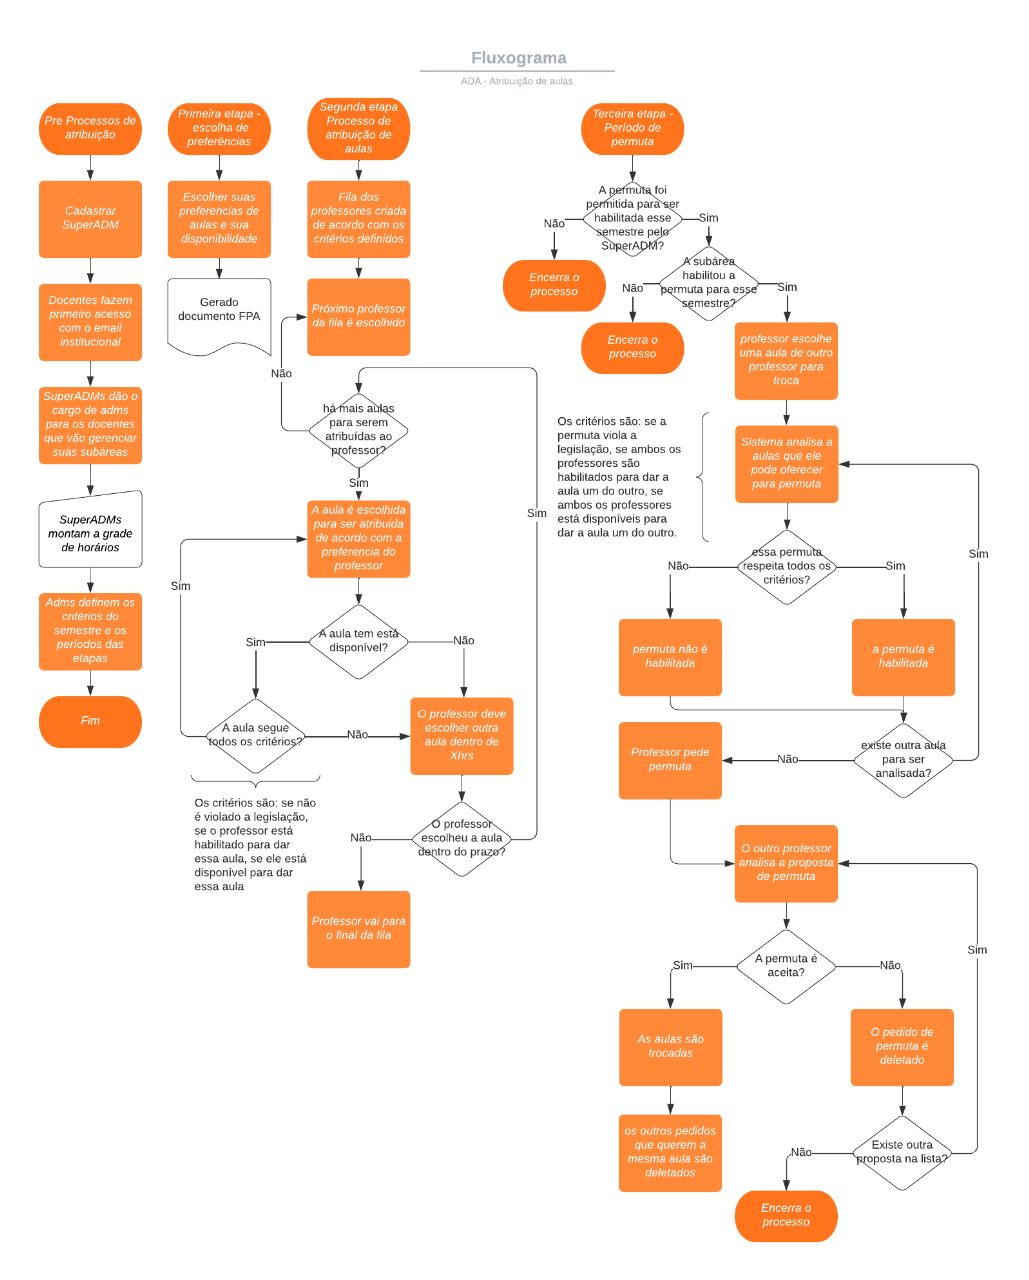
\includegraphics[width=0.8\textwidth]{fluxograma.jpeg}
    \caption{Primeira versão do fluxograma dos processos da ADA, para a PoC}
    \label{fig:diagrama}
\end{figure}

\subsection{Apêndice F - Testes automatizados}
\begin{figure}[h]
    \centering
    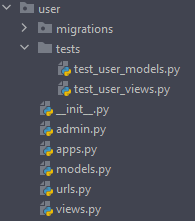
\includegraphics[width=0.5\textwidth]{arquivostestes.png}
    \caption{Exemplo das pastas com arquivos de testes}
    \label{fig:arquivostestes}
\end{figure}
\begin{figure}[h]
    \centering
    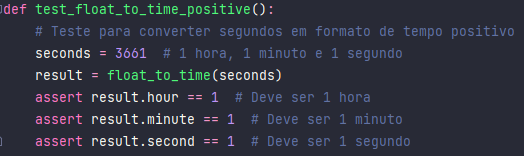
\includegraphics[width=0.8\textwidth]{funcaoteste.png}
    \caption{Exemplo da função teste com a verificação fornecida pelo Pytest}
    \label{fig:funcaoteste}
\end{figure}
\begin{figure}[h]
    \centering
    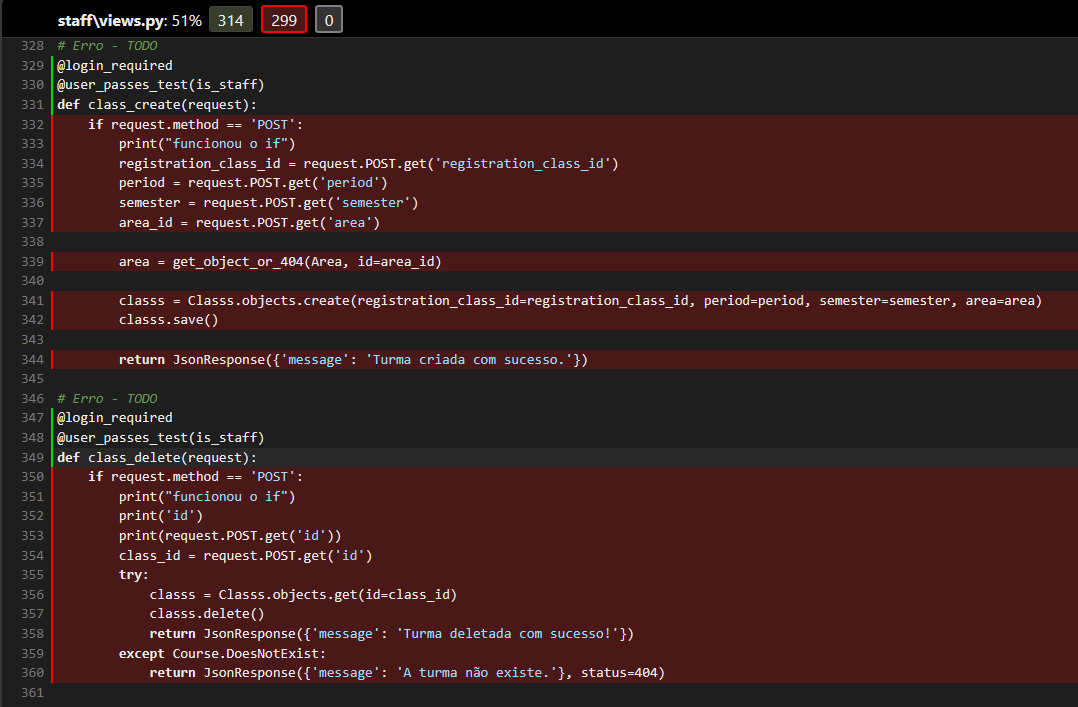
\includegraphics[width=0.9\textwidth]{testeerrado.png}
    \caption{Exemplo de uma verificação que indicou erros no código}
    \label{fig:testeerrado}
\end{figure}
\begin{figure}[h]
    \centering
    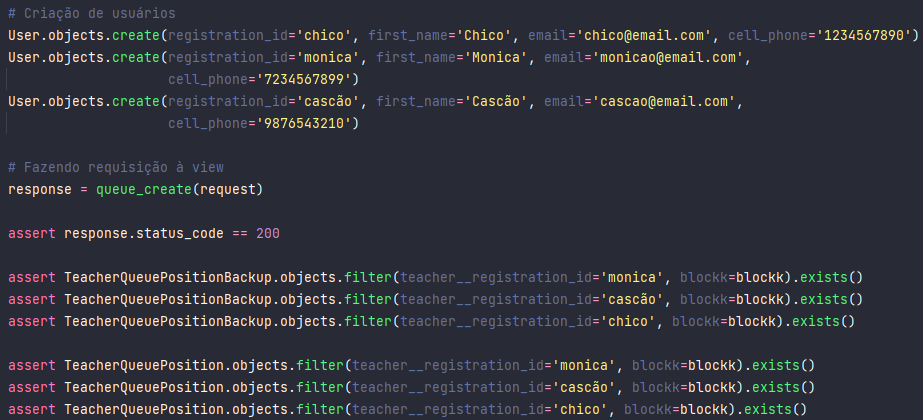
\includegraphics[width=0.9\textwidth]{classeficticia.png}
    \caption{Exemplo de uma classe fictícia}
    \label{fig:classeficticia}
\end{figure}
\begin{figure}[h]
    \centering
    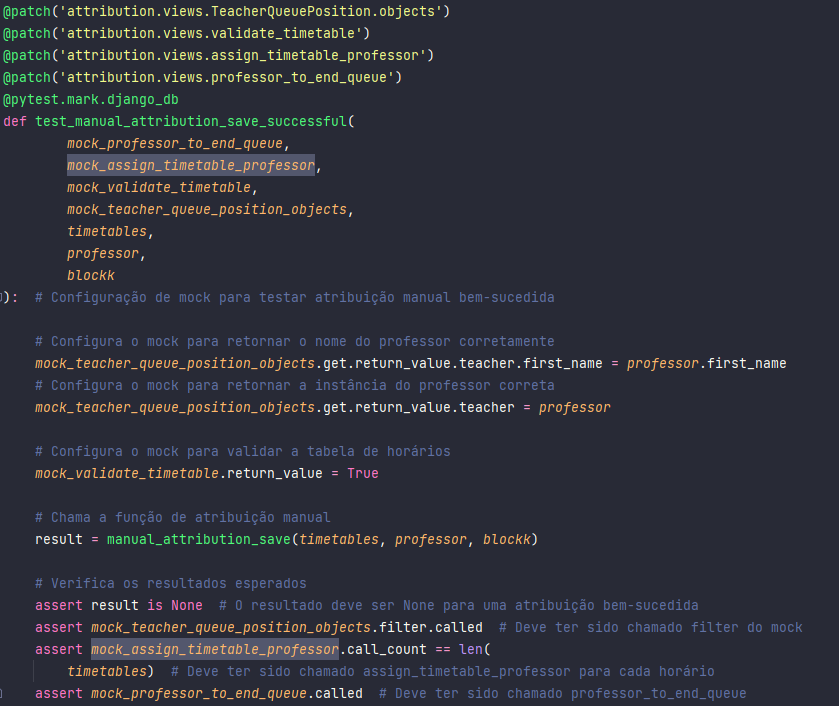
\includegraphics[width=0.9\textwidth]{funcaoficticia.png}
    \caption{Exemplo de uma função fictícia}
    \label{fig:funcaoficticia}
\end{figure}
\begin{figure}[h]
    \centering
    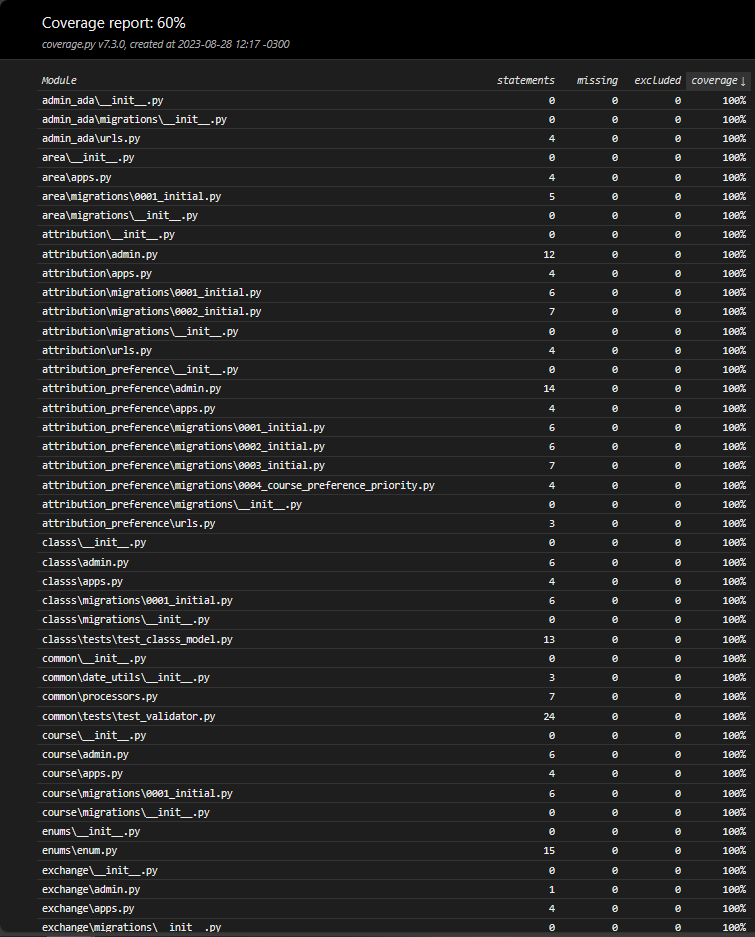
\includegraphics[width=1\textwidth]{coberturaparte1.png}
    \caption{Cobertura dos testes, indicada pela Pytest-cov - Parte 1}
    \label{fig:cobertura1}
\end{figure}
\begin{figure}[h]
    \centering
    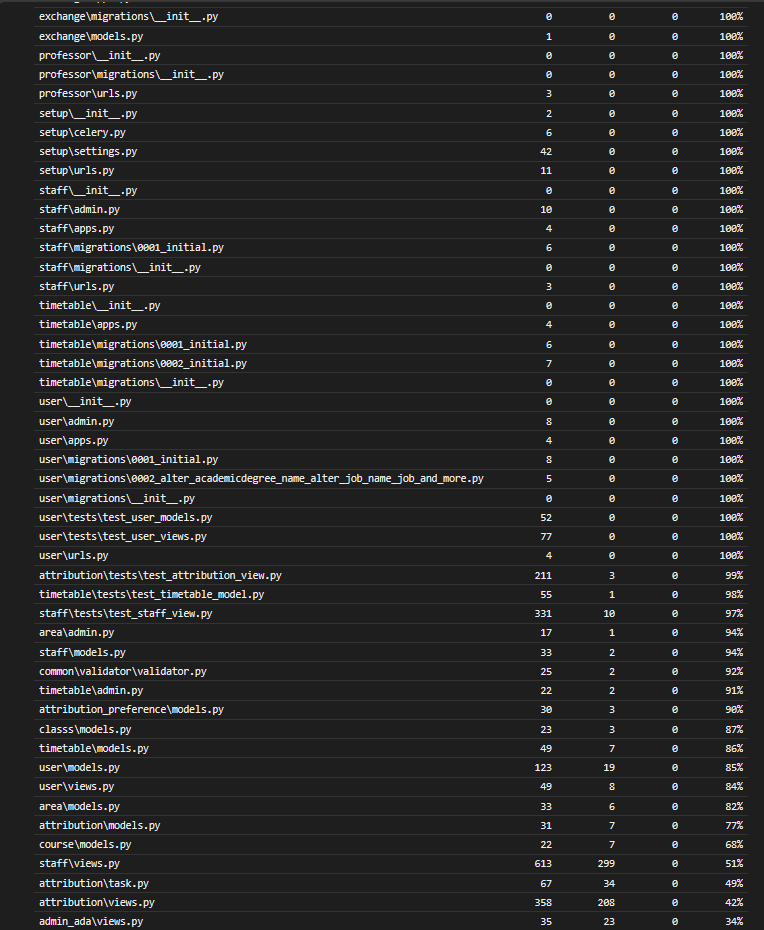
\includegraphics[width=1\textwidth]{coberturaparte2.png}
    \caption{Cobertura dos testes, indicada pela Pytest-cov - Parte 2}
    \label{fig:cobertura2}
\end{figure}
\begin{figure}[h]
    \centering
    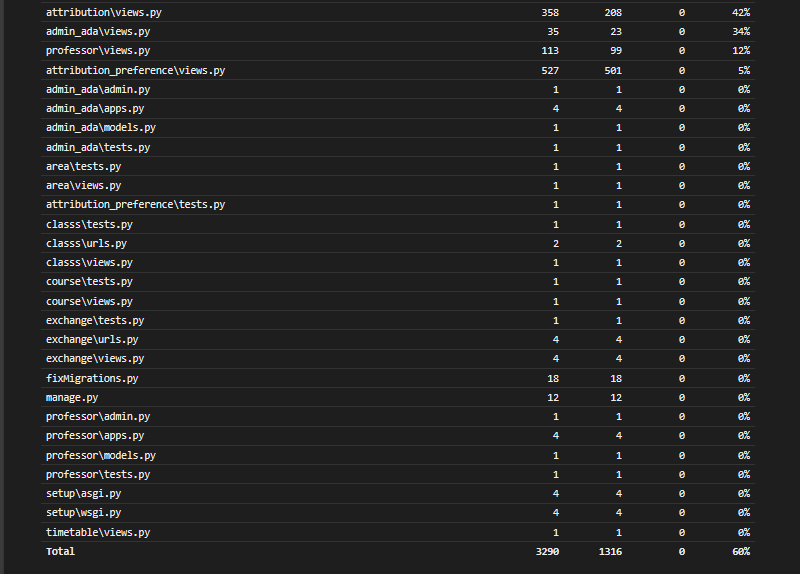
\includegraphics[width=1\textwidth]{coberturaparte3.png}
    \caption{Cobertura dos testes, indicada pela Pytest-cov - Parte 3}
    \label{fig:cobertura3}
\end{figure}
\begin{figure}[h]
    \centering
    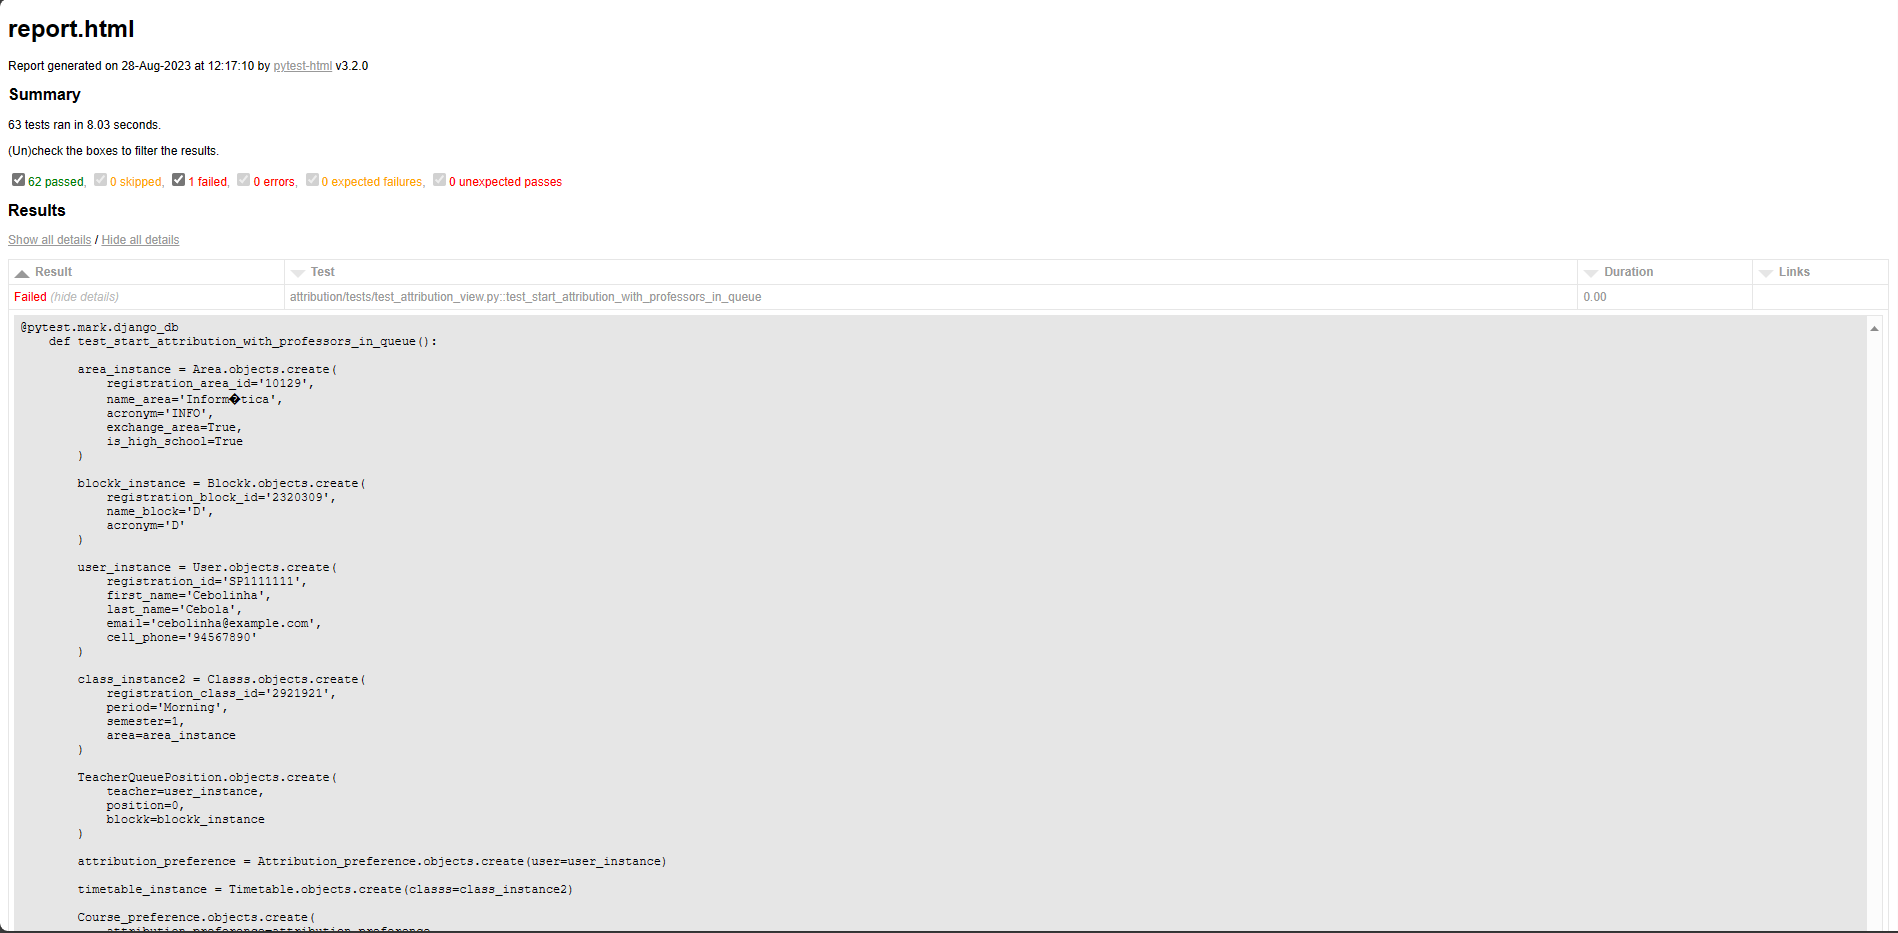
\includegraphics[width=1\textwidth]{relatorioparte1.png}
    \caption{Relatório dos testes - Parte 1}
    \label{fig:relatorio1}
\end{figure}
\begin{figure}[h]
    \centering
    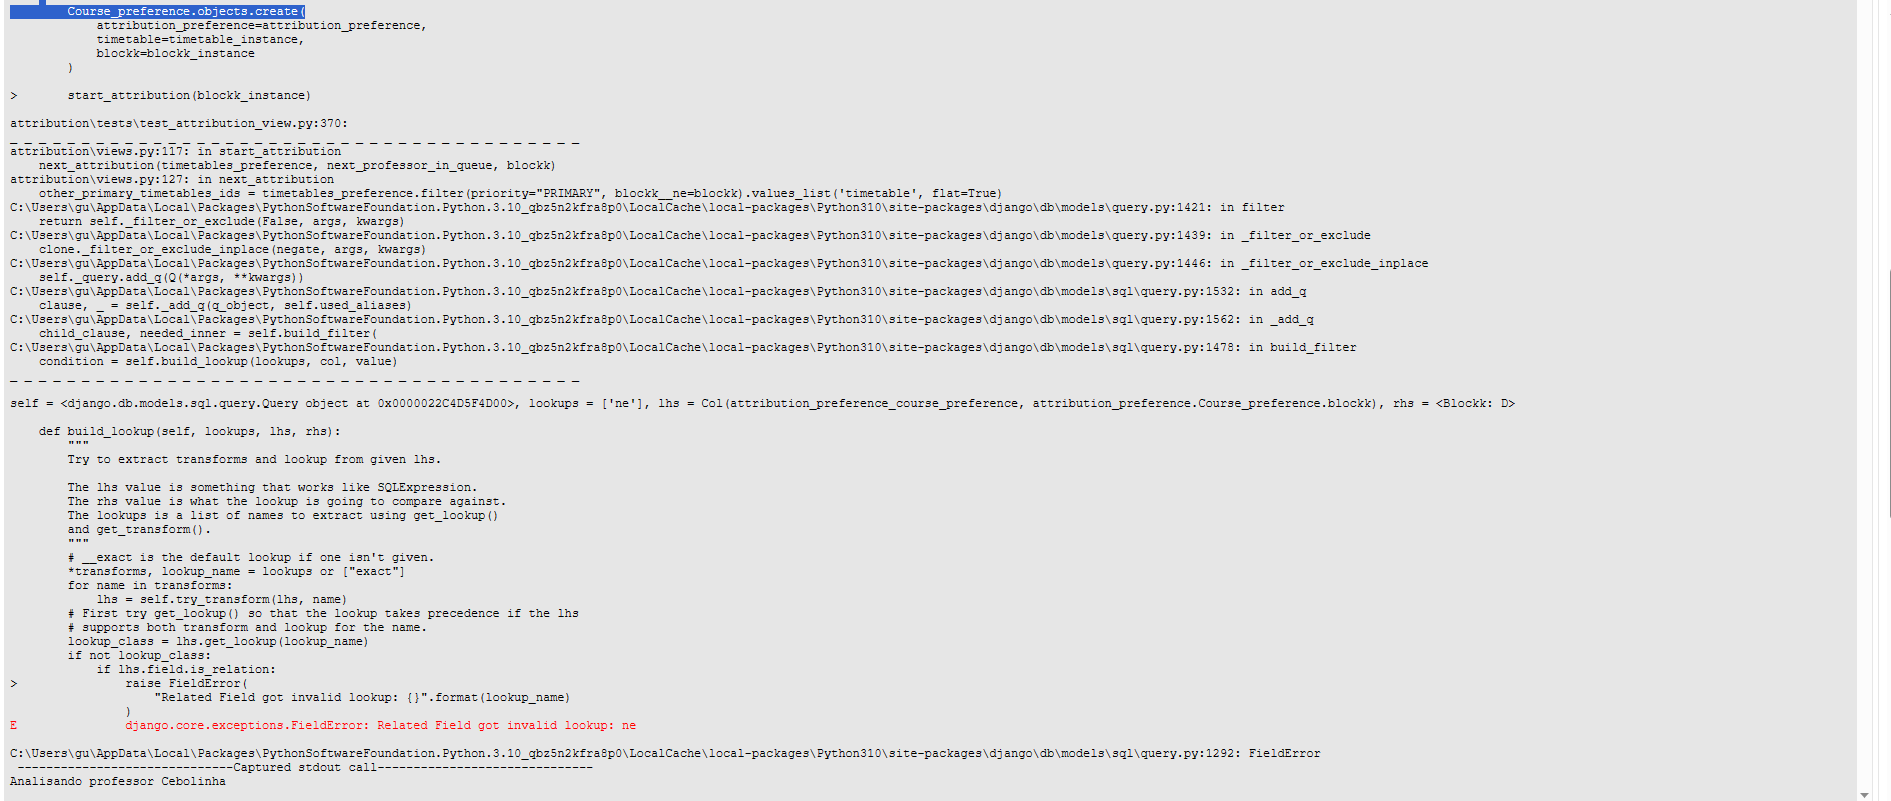
\includegraphics[width=1\textwidth]{relatorioparte2.png}
    \caption{Relatório dos testes - Parte 2}
    \label{fig:relatorio2}
\end{figure}
\begin{figure}[h]
    \centering
    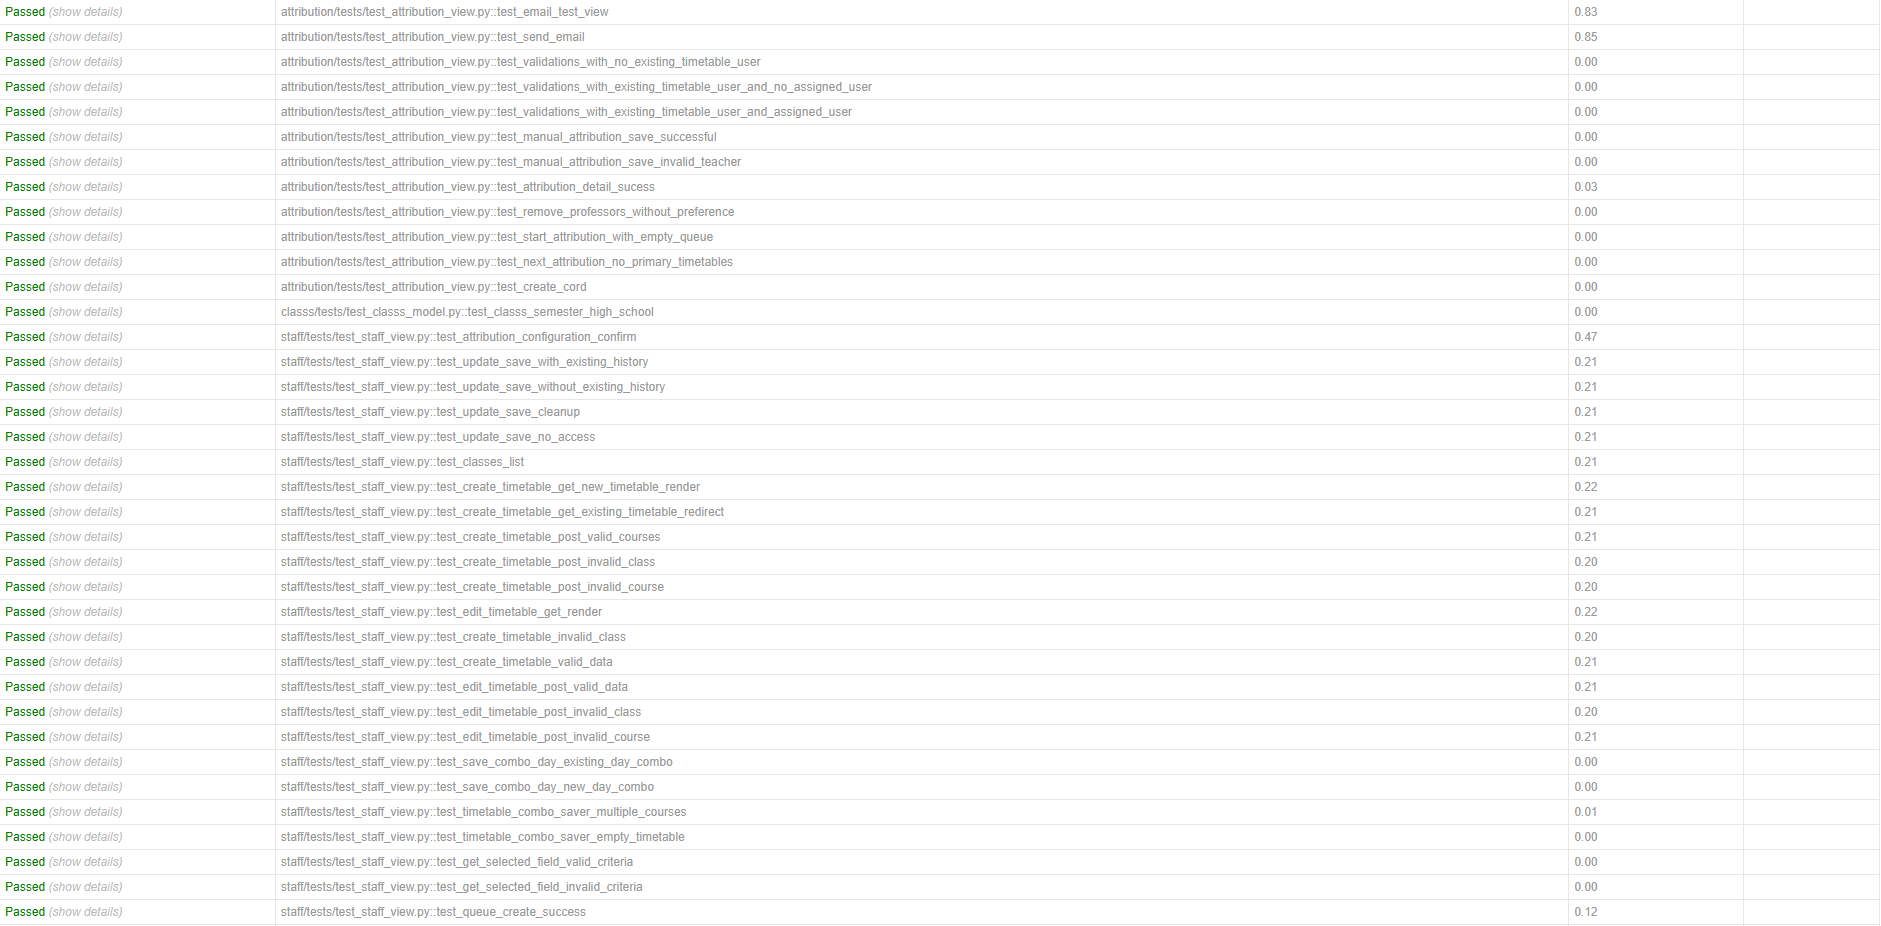
\includegraphics[width=1\textwidth]{relatorioparte3.png}
    \caption{Relatório dos testes - Parte 3}
    \label{fig:relatorio3}
\end{figure}
\begin{figure}[h]
    \centering
    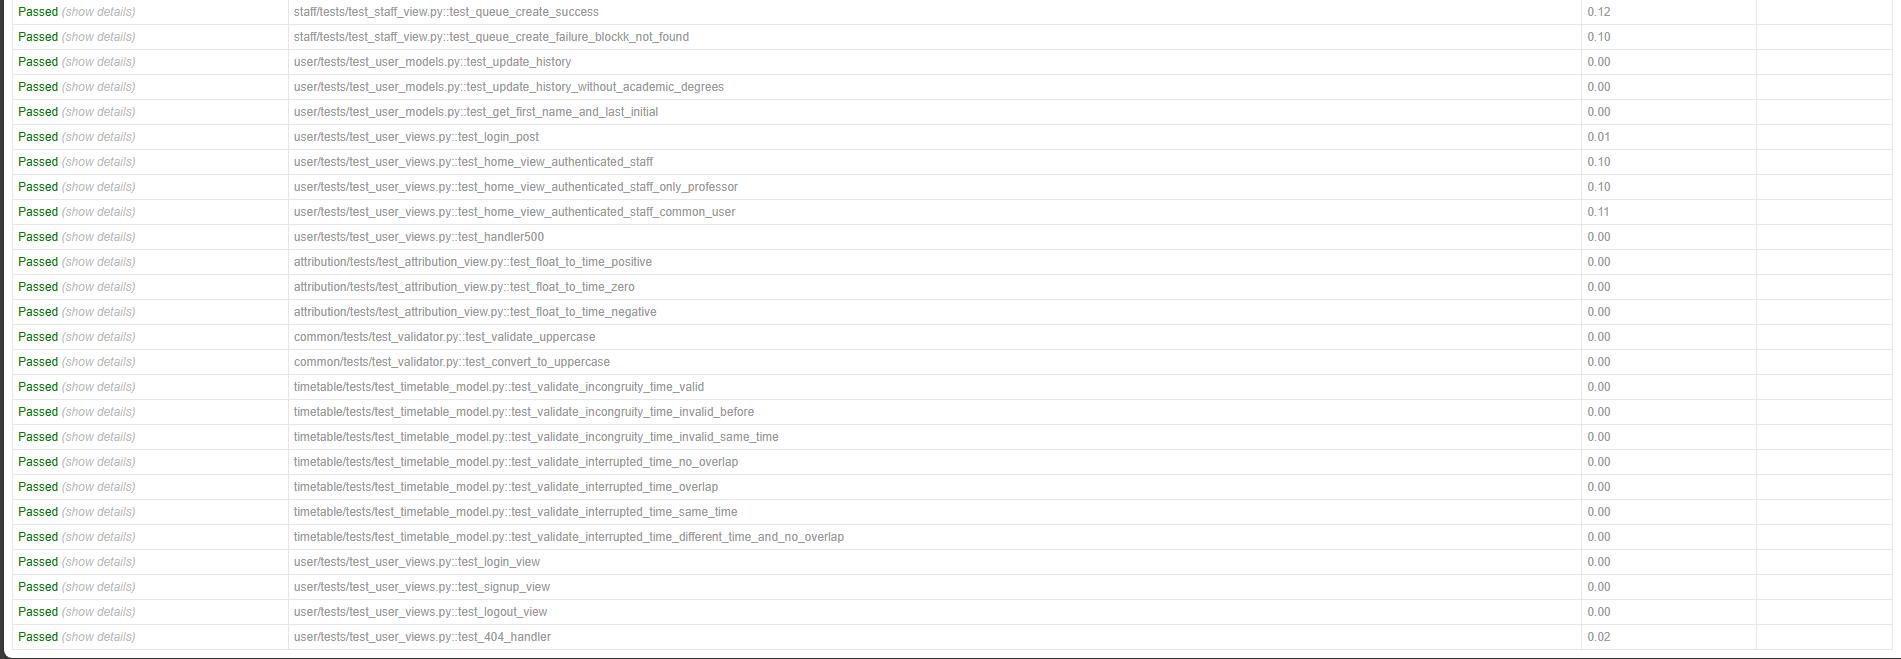
\includegraphics[width=1\textwidth]{relatorioparte4.png}
    \caption{Relatório dos testes - Parte 4}
    \label{fig:relatorio4}
\end{figure}


\end{document}
